\section{Chapter 3: Understanding the Risks and Benefits of Generative Models from the Perspective of Representation Learning}

\subsection{Overview}
In the first two chapters, we explore how powerful representations of data allow us to solve downstream tasks with greater efficiency and efficacy. We posed the geospatial representation learning problem as a neural field problem where we want to learn $R=F_\theta(lat, lon)$. Generative models pose a double-edged role in this landscape. On the positive side, they can be used to expand datasets through synthetic augmentation and unlock new possibilities for representation learning. The efficacy of representation learning scales with data and generative models can provide an easy alternative to scale pretraining. However, generative models also introduce the risk of contaminating training pipelines with low-quality data. Such contamination can mislead models into capturing spurious correlations, amplify existing biases, and ultimately yield representations that diverge from the true structure of the data. From this perspective, generative models are not simply tools for data creation but also potential vectors for introducing noise, bias, and adversarial artifacts into our neural representation fields. Understanding and mitigating these risks is, therefore, essential for building trustworthy and robust downstream models.

In Chapter 3, we will examine the potential risks and limitations of deep-generative geospatial models. First, we will demonstrate that current generative geospatial models introduce strong artifacts in the generated images. Second, we will propose a new metric that measures the strength of these artifacts in a given generative model. Third, we present SimLBR, a simple and efficient solution for detecting fake images in a real-world black-box setting, where the source of an image is unknown. SimLBR learns a tight decision boundary around the real image distribution using latent blending regularization, and generalizes to unseen generators on both natural-image and satellite-image benchmarks. We further extend SimLBR with structured latent blending strategies that improve its reliability on the hardest, most out-of-distribution generators. Finally, we will use the findings to propose better generative models that can feed into representation learning pipelines while maintaining the integrity and fidelity of the learned representations. By doing so, we aim to ensure that generative augmentation enhances rather than compromises the quality of downstream tasks, paving the way for robust, trustworthy, and scalable geospatial AI systems.

\subsection{Do Geospatial Generative Models Introduce Strong Artifacts in their Images?}
\label{sec:few-shot}
In this section, we will examine various geospatial generative models and assess the quality of the generated fakes. We will do this by using few-shot learning. Images that exhibit strong artifacts will be easier to detect compared to images that do not contain such artifacts. Hence, it should be possible to learn a good deepfake detector for models with strong artifacts, even when we only have access to a few samples.
\\
\\
\noindent \textbf{Dataset:}
We will use the RSFAKE-1M data, a large-scale dataset for detecting diffusion-generated remote sensing forgeries~\cite{tan2025rsfake}. The dataset contains 500,000 real and 500,000 forged satellite images. The forged images are obtained from 10 different diffusion models that are trained on remote sensing images. 
\\
\\
\noindent\textbf{Experimental Setup:} 
Assume we have real images from set $R$, and fake images from set $F$. All images in $F$ are generated from the same model. We want to understand if it is possible to identify all samples in $F$, if we only have access to a subset of $F$, $G$ with n fake images during training (where n is very small).

During training, we have access to $R=\{r_1, r_2, ..., r_k\}$, and $G=\{g_1, g_2, ...g_n\}$. All the real images are passed through a powerful, pre-trained satellite image encoder $I$, which produces the set of real features $R_f$. Since $\lvert R \lvert >> \lvert G \lvert$, we apply multiple augmentations to $g_i$, and artificially increase the number of fake samples. All of the fake samples are then passed through the pre-trained satellite image encoder $I$, which produces the set of generated image features $G_f$. We then train a simple linear binary classifier to distinguish between real and fake images.
\\
\\
\begin{table*}[]
\resizebox{\linewidth}{!}{
\begin{tabular}{llll|lll|lll|lll}
\multicolumn{1}{r}{} & \multicolumn{3}{c|}{100 samples} & \multicolumn{3}{c|}{10 samples} & \multicolumn{3}{c|}{2 samples} & \multicolumn{3}{c}{1 sample} \\ \hline
                     & Acc   & Auc   & \multicolumn{1}{l|}{F1} & Acc   & Auc   & \multicolumn{1}{l|}{F1} & Acc   & Auc   & \multicolumn{1}{l|}{F1} & Acc   & Auc   & F1 \\ \hline
Geosynth         & 0.999 & 0.999 & 0.999 & 0.998 & 0.999 & 0.998 & 0.979 & 0.997 & 0.979 & 0.969 & 0.995 & 0.969 \\
Geosynth-SAM     & 0.999 & 0.999 & 0.999 & 0.997 & 0.999 & 0.997 & 0.986 & 0.999 & 0.986 &    0.986   &    0.999   &   0.986   \\
Rsinpaint        & 0.969 & 0.997 & 0.969 & 0.931 & 0.986 & 0.928 & 0.877 & 0.964 & 0.863 & 0.775 & 0.908 & 0.725 \\
GeoRSSD (fmow)       & 0.997 & 0.999 & 0.997 & 0.992 & 0.999 & 0.992 & 0.988 & 0.999 & 0.988 & 0.979 & 0.998 & 0.979 \\
MapSat           & 0.999 & 0.999 & 0.999 & 0.996 & 0.999 & 0.996 & 0.995 & 0.999 & 0.995 & 0.845 & 0.979 & 0.819 \\
DiffusionSat-512 (fmow) & 0.994 & 0.999 & 0.994 & 0.986 & 0.999 & 0.985 & 0.943 & 0.991 & 0.941 & 0.890 & 0.976 & 0.881 \\
DiffusionSat-256 (fmow) & 0.995 & 0.999 & 0.995 & 0.989 & 0.999 & 0.989 & 0.967 & 0.994 & 0.967 & 0.854 & 0.967 & 0.836 \\
CrsDiff (fmow) & 0.997 & 0.999 & 0.997 & 0.968 & 0.997 & 0.968 & 0.908 & 0.989 & 0.900 & 0.606 & 0.831 & 0.368 \\
SDFRS            & 0.999 & 0.999 & 0.999 & 0.999 & 0.999 & 0.999 & 0.978 & 0.998 & 0.977 & 0.982 & 0.999 & 0.981 \\


\end{tabular}
}
\caption{A linear classifier with few-shot examples yields good results in detecting geospatial deepfakes.}
\label{table:few-shot}
\end{table*}
\noindent\textbf{Preliminary Results:}
We conduct this experiment for each model in the RSFAKE-1M dataset. We report the results for $n=\{100,10,2,1\}$. The results are reported in Table~\ref{table:few-shot}. The preliminary results show that it is possible to learn a strong binary classifier with access to as few as one fake sample from a generative model. This leads us to make two crucial hypotheses:
\begin{enumerate}
    \item Every image generated from a model contains artifacts that are, in part or in whole, shared by any other images generated from the same model.
    \item Including images with such strong artifacts for training new models will result in biased models and biased representations.
\end{enumerate}
We will design methods to validate these hypotheses experimentally.

\subsection{A New Metric to Understand the Presence of Artifacts in Geospatial Deepfakes}
\label{sec:seperability}
Based on our findings in Section~\ref{sec:few-shot}, we will propose a new metric to measure the performance of a geospatial generative model. Our metric measures, ``for a generative model $G$, how many randomly-sampled fake images are needed to learn a linear classifier that gets an accuracy of K on an unseen test set". The linear classifier is learned using the protocol described in Section~\ref{sec:few-shot}. When comparing different models, the same feature extractor must be used for a fair comparison. For a generative model, a lower value of Separability indicates that the model introduces trivial artifacts in all images that it produces. In contrast, a higher value suggests that artifacts are less prevalent. We will compute the Separability value for the state-of-the-art generative models to have a better understanding of which models can be used to generate synthetic data with minimal risks. 

\subsection{SimLBR: Learning to Detect Fake Images by Learning to Detect Real Images}
\label{sec:simlbr}
The few-shot experiments in Section~\ref{sec:few-shot} show that a detector can be trained to recognize the fakes of a \textit{known} generator from only a handful of samples. In practice, however, the source of an image is unknown, and the generator that produced a fake image may not have existed when the detector was trained. While it is relatively easy to train a detector that performs well on fakes produced by a specific generative model, real-world deployment demands detectors that generalize to unseen and more advanced generators~\cite{ojha2023towards,yansanity,zhong2023patchcraft}. Unfortunately, most existing detectors overfit, learning superficial cues that are specific to the training generator rather than generalizable differences between real and fake images, and their performance collapses on images synthesized by novel generators. In this section, we present SimLBR~\cite{dhakal2026simlbr}, a simple and efficient framework for generalizable fake image detection using Latent Blending Regularization (LBR). Although our motivation comes from geospatial generative models, the problem of cross-generator generalization is not specific to satellite imagery. We therefore develop and evaluate SimLBR on standard natural-image benchmarks, and additionally evaluate it on the RSFake-1M benchmark of generated satellite images~\cite{tan2025rsfake}.

\noindent\textbf{From SimDLR to SimLBR:}
Our preliminary formulation of this idea, SimDLR, aimed to prevent overfitting by \textit{diversifying the artifacts} seen during training: each fake embedding was linearly combined with the embedding of another randomly sampled real or fake image, and the combination was labeled as fake. While this improved cross-generator generalization on RSFake-1M, it still asks the detector to model the \textit{fake} distribution, which is a moving target. In SimLBR, we reverse the role of the two classes. Instead of enlarging the region of the latent space that is covered by fake samples, we perturb \textit{real} samples with small amounts of fake information and label them as fake. This forces the detector to learn a tight decision boundary around the real image distribution and to treat the fake category as a sink class. The rest of this section describes this formulation in detail.

\begin{figure}[!t]
\centering
\begin{minipage}[t]{0.48\linewidth}
  \centering
  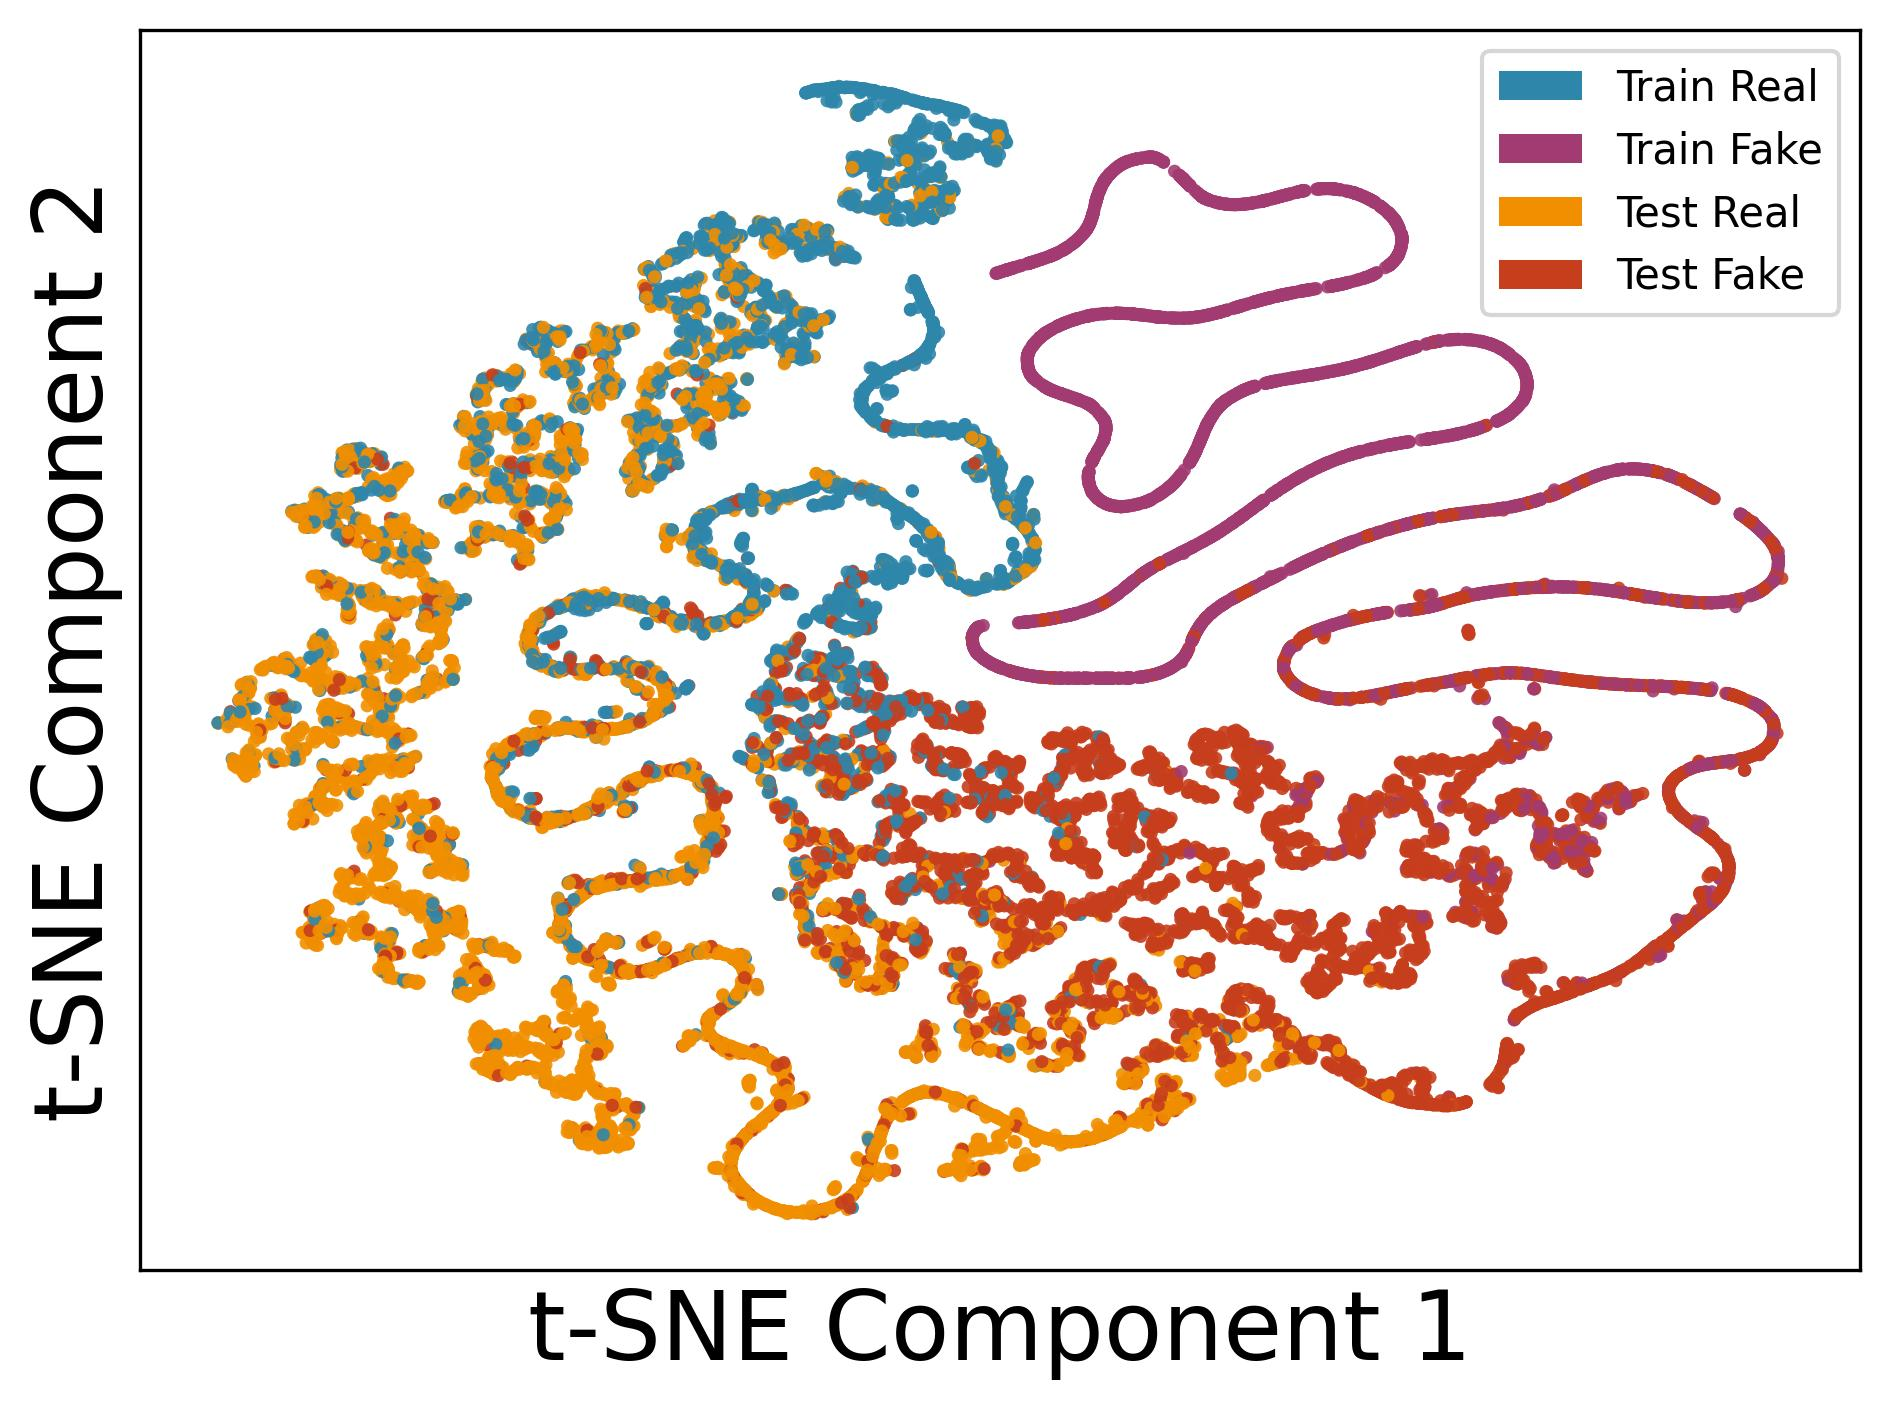
\includegraphics[width=\linewidth]{proposal/images/simlbr/tsne_wo_lbr_wukong.jpeg}\\
  {\small (a) w/o LBR}
\end{minipage}\hfill
\begin{minipage}[t]{0.48\linewidth}
  \centering
  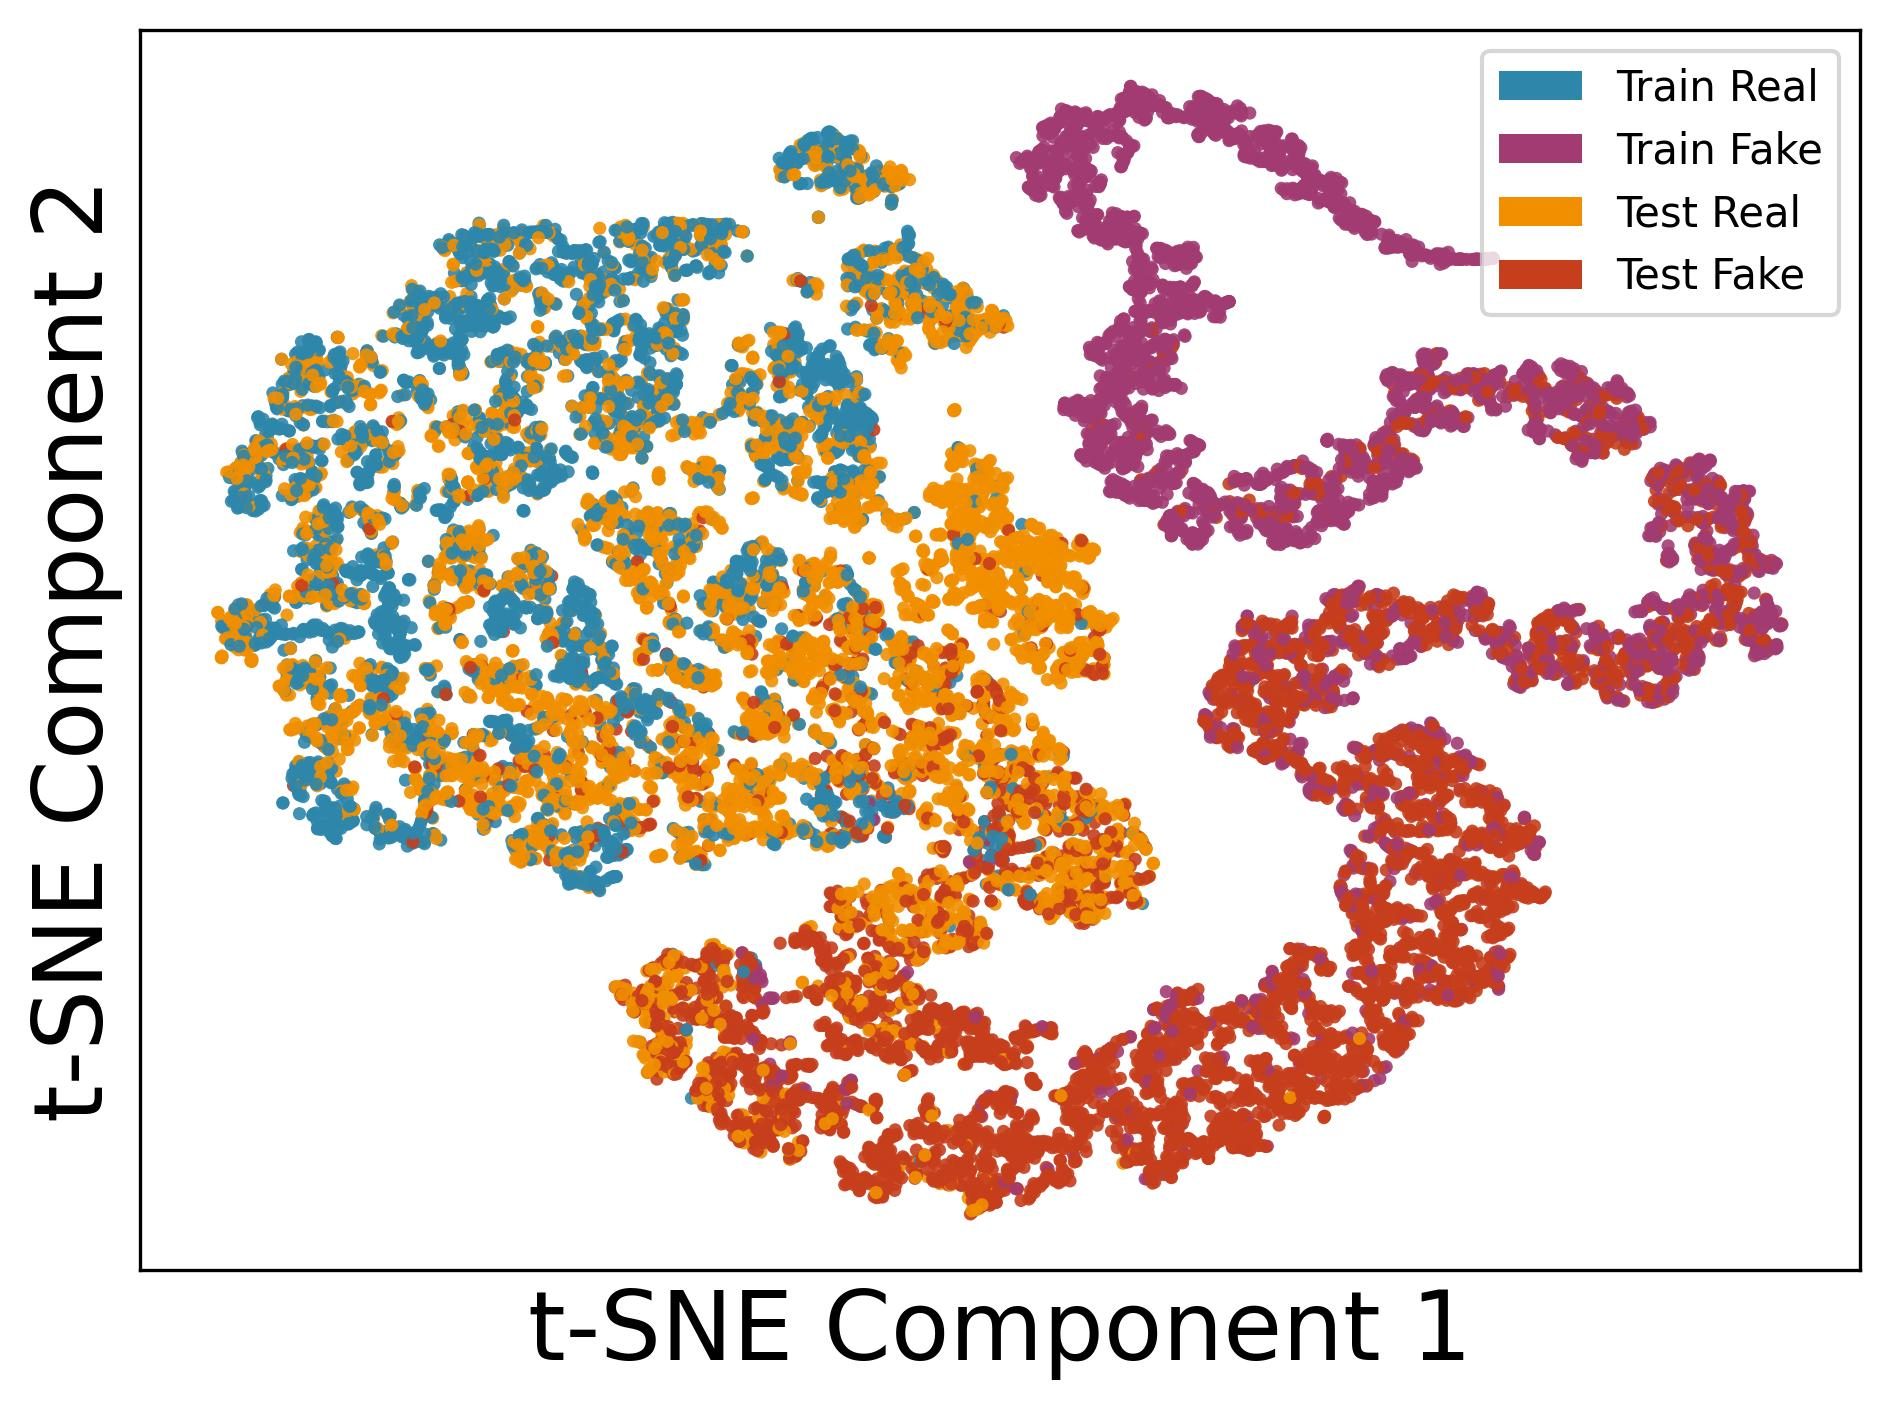
\includegraphics[width=\linewidth]{proposal/images/simlbr/tsne_w_lbr_wukong.jpeg}\\
  {\small (b) w/ LBR}
\end{minipage}
\caption{\textbf{t-SNE visualization of Latent Blending Regularization:} Detectors trained without LBR overfit to generator-specific artifacts, so fake images from an unseen generator (Wukong, red points) are misclassified as real. With LBR, the detector learns a tight boundary around the real image distribution (blue/orange cluster), and any sample outside this region, regardless of its generative source, is classified as fake. The detector is trained on ProGAN images.}
\label{fig:simlbr_tsne}
\end{figure}

\subsubsection{Fake Image Detection as Learning a Tight Boundary Around Real Images}
Ojha et al.~\cite{ojha2023towards} showed that, during training, most detectors learn to identify generator-specific fingerprints rather than the underlying distributional differences between real and fake images. When these fingerprints are absent from a new generator, the detector classifies its fakes as real, effectively treating the real category as a \textit{sink class}: a class that absorbs all out-of-distribution samples regardless of their true label. This behavior was further highlighted by AIDE~\cite{yansanity}, which argued that common benchmarks such as AIGC~\cite{wang2020cnn} and GenImage~\cite{zhu2023genimage} contain randomly generated images with no guarantee of perceptual quality, and introduced Chameleon, a test set of fake images that pass a human perception \textit{Turing Test}. State-of-the-art detectors, including UnivFD~\cite{ojha2023towards} and AIDE~\cite{yansanity}, degrade severely on Chameleon, and the degradation is caused primarily by fake images being classified as real.

Learning a tight boundary around the fake samples seen during training is highly undesirable, because the distribution of fake images is continually evolving. New generative models with completely different structures and artifacts are constantly introduced, pushing their samples outside the learned boundary. In contrast, the distribution of real images remains relatively stable. Shifts caused by improved camera sensors are minor and occur over long periods of time. We therefore propose that fake image detection should be solved by learning a tight boundary around the \textit{real} image distribution and using the fake category as the sink class. Intuitively, anything that is not real can be placed in the fake category, irrespective of the nature and origin of the fake sample.

One way to model only the real distribution is to frame the problem as anomaly detection~\cite{scholkopf2001ocsvm,ruff2018deep,hendrycks2017baseline}. However, in the extremely high-dimensional space of natural images, the assumption that photorealistic fakes will naturally fall outside the learned real-image manifold is unrealistic. We verify this in Section~\ref{sec:simlbr_ablation}, where a One-Class SVM trained on the same features substantially underperforms SimLBR. Effective discrimination therefore requires training signals derived from fake images that guide the model toward a meaningful boundary. Several face-forgery detectors~\cite{nguyen2024laa,Shiohara_2022_CVPR,tian2024real} construct pseudo-fakes by applying hand-crafted manipulations to real images. However, these methods operate in pixel space, often require task-specific preprocessing such as facial landmark detection, and introduce only a narrow family of low-level artifacts. SimLBR instead constructs pseudo-fakes in the latent space of a pretrained foundation model, using guidance from real fake images.

\subsubsection{Measuring Reliability and Worst-Case Performance}
\label{sec:reliability}
Most fake image detection works report average accuracy across generators as the key measure of performance. However, detectors often exhibit high variance across generators: a model may achieve over 99\% accuracy on one generator and drop to nearly 50\% on another. The true utility of a detector lies in its robustness to the next generation of models that are unknown at training time, so the variance across generators is a critical dimension of evaluation. To quantify the trade-off between accuracy and stability, we adapt the Sharpe ratio~\cite{sharpe1994ratio}, which measures excess return relative to risk, and define the \textit{Reliability} of a detector as:
\begin{equation}
\text{Reliability} = \frac{\mu_{\text{acc}} - A_{\text{base}}}{\sigma_{\text{acc}}}
\label{eq:reliability}
\end{equation}
where $\mu_{\text{acc}}$ is the mean accuracy across all evaluated generators, $\sigma_{\text{acc}}$ is the corresponding standard deviation, and $A_{\text{base}}$ is the accuracy of a naive ``risk-free'' baseline. We set $A_{\text{base}}=50$, the accuracy of a random predictor. A higher reliability indicates a detector that is both accurate and stable across generators.

We additionally report a \textit{Worst-Case Estimate} (WCE), defined as the lowest accuracy of a detector across all evaluated generators. This quantity approximates the performance of the detector when confronted with a future generator that deviates most from the training distribution, and serves as an upper bound on its true worst-case performance in the open world.

\begin{figure}[!t]
\begin{center}
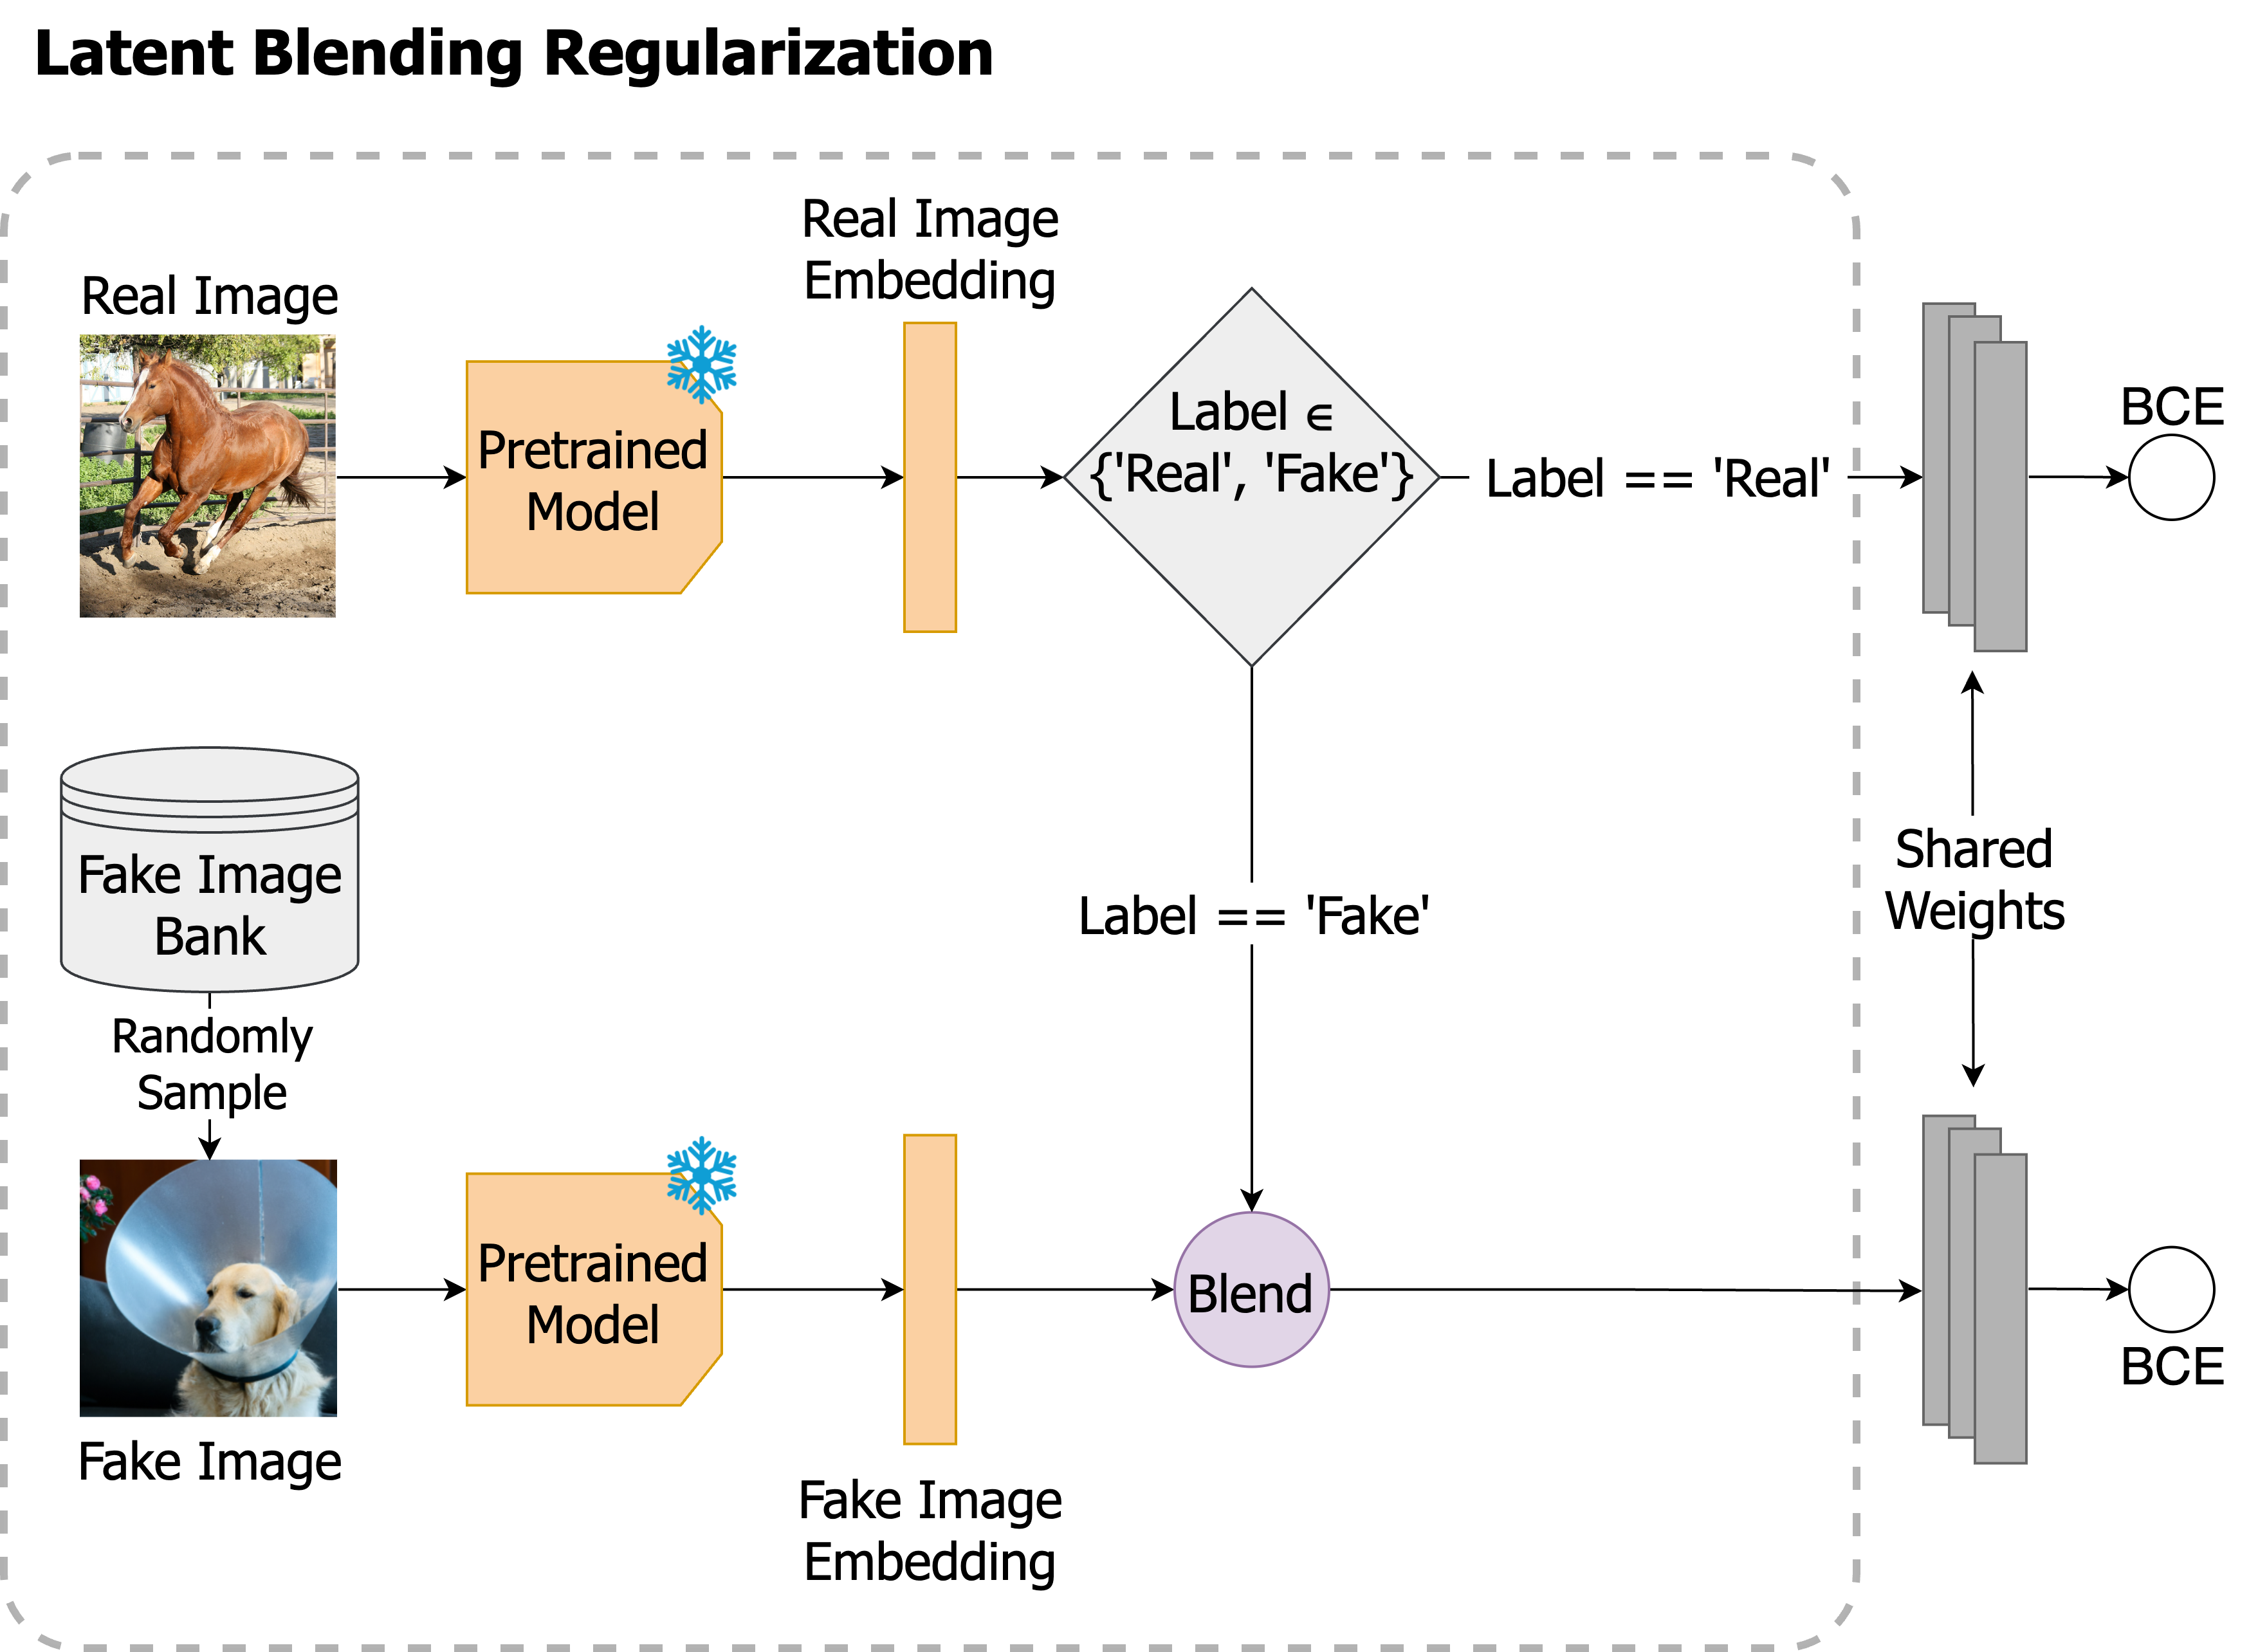
\includegraphics[width=\linewidth]{proposal/images/simlbr/simlbr_framework.png}
\end{center}
\caption{\textbf{Framework of SimLBR:} For each real image in the training set, the model samples either a real or a fake label. If a fake label is sampled, a small amount of fake image information is blended into the real image representation in a pretrained latent space. Solving this objective forces the model to learn a tight decision boundary around the unperturbed real image distribution, enabling better generalization to unseen generative models.}
\label{fig:simlbr_framework}
\end{figure}

\begin{figure}[!t]
\begin{center}
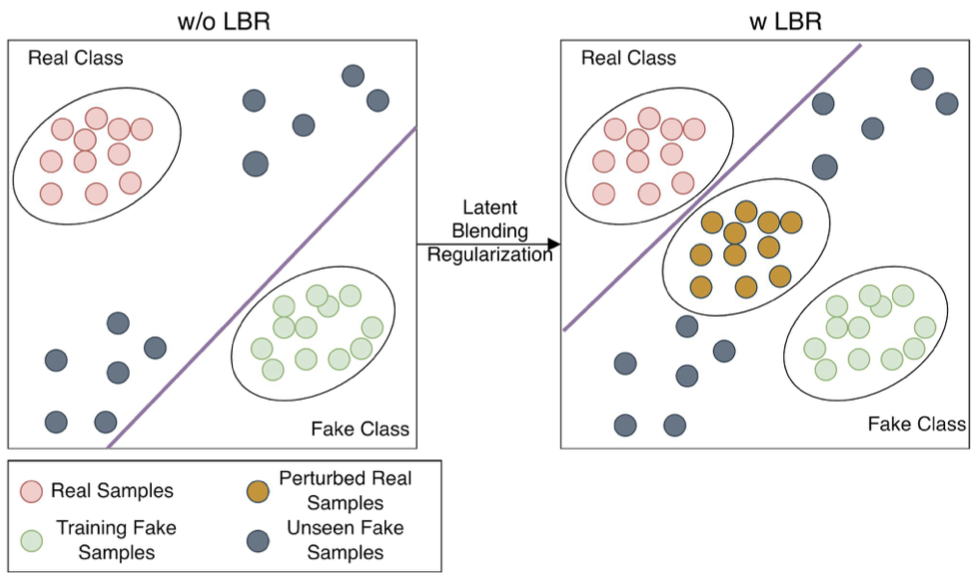
\includegraphics[width=0.85\linewidth]{proposal/images/simlbr/lbr_boundary_schematic.png}
\end{center}
\caption{\textbf{Intuition behind Latent Blending Regularization:} Without LBR (left), the detector learns a boundary that tightly encloses the training fakes, so unseen fakes fall on the real side of the boundary. LBR introduces perturbed real samples (yellow) that lie just outside the real distribution and are labeled as fake. This pushes the decision boundary toward the real distribution (right), so that unseen fakes from any generator are classified as fake.}
\label{fig:lbr_schematic}
\end{figure}

\subsubsection{Method}
Following prior work, we train on fake images from a single source generator $G_s$ and evaluate on a set of unseen generators $\mathbb{U}=\{U_1, U_2, \ldots, U_m\}$. Let $\mathbb{R}=\{R_1, R_2, \ldots, R_n\}$ be the set of real training images, $\mathbb{F}=\{F_1, F_2, \ldots, F_n\}$ the set of fake training images, and $I$ a frozen, pretrained image feature extractor. During training, a real image $R_i$ is sampled and assigned a random label $y_i \in \{0,1\}$. If $y_i=0$, its features are computed as $L_i = I(R_i)$. If $y_i=1$, we compute its features using Latent Blending Regularization.

\noindent\textbf{Latent Blending Regularization (LBR):} For a real image $R_i$ with label $y_i=1$, we randomly sample a fake image $F_i$ from the training set and compute the features of both images:
\begin{equation}
L_i^{R} = I(R_i), \qquad L_i^{F} = I(F_i)
\label{eq:lbr_features}
\end{equation}
The final representation is a linear interpolation between the two latent representations:
\begin{equation}
L_i = \alpha L_i^{R} + (1-\alpha) L_i^{F}
\label{eq:lbr}
\end{equation}
The overall training setup is summarized in Figure~\ref{fig:simlbr_framework}, and the intended effect on the decision boundary is illustrated in Figure~\ref{fig:lbr_schematic}. The key idea is that even a small injection of fake information into a real image should be classified as fake. This forces the detector to recognize only completely unaltered, truly authentic images as real, thereby compelling it to model the structure of the real distribution.

Blending in the latent space of a pretrained model, rather than in pixel space~\cite{zhang2018mixup}, is central to our approach and differs from prior blending strategies in both motivation and formulation~\cite{Shiohara_2022_CVPR,verma2019manifold}. First, perturbed samples are constructed efficiently through simple vector arithmetic. Second, $\alpha$ gives fine-grained control over the amount of fake information that is injected, enabling a virtually unlimited number of perturbed real samples. Most importantly, blending in a semantic latent space keeps the classification of real images non-trivial. When blending occurs in pixel space, low-level artifacts can be copied directly from the fake image, and the model can identify perturbed samples by detecting these artifacts. Latent-space blending operates on higher-level representations where such low-level cues are less likely to be preserved, forcing the detector to learn meaningful distinctions and enforce a tighter boundary around the real distribution. We use DINOv3~\cite{simeoni2025dinov3}, whose expressive representations preserve high-level structure and semantics, enabling meaningful interpolation between real and fake samples.

\noindent\textbf{Sampling distribution for $\alpha$:} The choice of sampling distribution for $\alpha$ directly determines how effectively the regularizer makes real-image classification non-trivial. Low values of $\alpha$ inject a large proportion of fake information, producing representations that are trivially identified as fake. Conversely, extremely high values of $\alpha$ (e.g., $\alpha=0.99$) produce blended representations that are almost indistinguishable from real samples, forcing the model to separate nearly identical embeddings into different classes, which is an unstable training scenario. We adopt the intuition that a meaningful perturbed real sample should retain the majority of the information from the real image while incorporating only a small proportion from the fake image. Accordingly, we sample:
\begin{equation}
\alpha \sim \text{Uniform}(0.5, B)
\label{eq:alpha_sampling}
\end{equation}
where $B$ is an upper bound. We verify this choice with an ablation study in Section~\ref{sec:simlbr_ablation}.

\noindent\textbf{Training objective:} The features are passed through a lightweight MLP $F_\theta$, which is trained with the Binary Cross-Entropy (BCE) objective:
\begin{equation}
\mathcal{L}_{\text{BCE}} = -\frac{1}{N} \sum_{i=1}^{N} \left[ y_i \log F_{\theta}(L_i) + (1 - y_i) \log\left(1 - F_{\theta}(L_i)\right) \right]
\label{eq:simlbr_bce}
\end{equation}
For implementation simplicity, instead of resampling labels for the same real image, we iterate over the entire training set and, whenever a fake image is encountered, sample a real image to form a pair and assign the blended representation a fake label. This pairing ensures that all real and fake training samples are used.

\subsubsection{Experimental Setup}
\noindent\textbf{Implementation details:} We use DINOv3~\cite{simeoni2025dinov3} as the feature extractor in all experiments. For efficiency, we precompute embeddings for the entire training set and train a two-layer MLP classifier with ReLU activations on these features. SimLBR is trained with a batch size of 500 for a maximum of 10 epochs, with the upper bound $B$ of the $\alpha$ distribution set to $0.8$. We use the Adam optimizer with a learning rate of \texttt{1e-4} and weight decay of \texttt{1e-2}. After embeddings are precomputed, a training run requires approximately 3 minutes on a single NVIDIA H100 GPU. Precomputing the embeddings takes around 50 minutes for the AIGC and 22 minutes for the GenImage training sets. For comparison, the previous state-of-the-art method, AIDE~\cite{yansanity}, was trained on eight NVIDIA A100 GPUs for roughly two hours.

\noindent\textbf{Datasets:} We follow the standard cross-generator protocol: the detector is trained on fake images from a single generator and evaluated on images from a set of unseen generators. We evaluate on four benchmarks:
\begin{itemize}
    \item \textbf{GenImage}~\cite{zhu2023genimage}: we train on Stable Diffusion v1.4~\cite{rombach2022high} and evaluate on 7 other generators.
    \item \textbf{AIGC}~\cite{wang2020cnn}: we train on ProGAN~\cite{karras2017progressive} and evaluate on 15 other generators.
    \item \textbf{Chameleon}~\cite{yansanity}: a curated hard test set of fake images that pass a human perception test. We evaluate models trained on ProGAN and on Stable Diffusion v1.4.
    \item \textbf{RSFake-1M}~\cite{tan2025rsfake}: 500,000 real and 500,000 synthetic satellite images from 10 satellite-specific diffusion models (DiffusionSat-512, DiffusionSat-256~\cite{khanna2024diffusionsat}, GeoRSSD, SDFRS, GeoSynth-Text, GeoSynth-SAM, GeoSynth-Canny, CRSDiff, MapSat, and RSPaint). We train on DiffusionSat-512 and DiffusionSat-256 and evaluate on held-out test sets from all ten models. For this benchmark, we use the DINOv3-Satellite backbone, which is pretrained on 493M satellite images.
\end{itemize}
Along with average accuracy, we report the standard deviation across generators, the reliability score (Equation~\ref{eq:reliability}), and the worst-case estimate.

\begin{table*}[!t]
\resizebox{\linewidth}{!}{
\begin{tabular}{l|c|ccccccc|ccc}
Method & \begin{tabular}[c]{@{}c@{}}SD v1.4\\ (Training)\end{tabular} & Midjourney & SD v1.5 & ADM & GLIDE & Wukong & VQDM & BigGAN & \textit{Mean}$\uparrow$ & \textit{Std}$\downarrow$ & \textit{Rel.}$\uparrow$ \\
\hline
ResNet-50  & \textbf{99.90} & 54.90 & 99.70 & 53.50 & 61.90 & 98.20 & 56.60 & 52.00 & 72.09 & 22.70 & 0.97 \\
DeiT-S     & \textbf{99.90} & 55.60 & 99.80 & 49.80 & 58.10 & 98.90 & 56.90 & 53.50 & 71.56 & 23.29 & 0.92 \\
Swin-T     & \textbf{99.90} & 62.10 & 99.80 & 49.80 & 67.60 & 99.10 & 62.30 & 57.60 & 74.78 & 21.17 & 1.17 \\
CNNSpot    & 96.30 & 52.80 & 95.90 & 50.10 & 39.80 & 78.60 & 53.40 & 46.80 & 64.21 & 22.63 & 0.62 \\
Spec       & 99.40 & 52.00 & 99.20 & 49.70 & 49.80 & 94.80 & 55.60 & 49.80 & 68.79 & 24.14 & 0.77 \\
F3Net      & \textbf{99.90} & 50.10 & \underline{99.90} & 49.90 & 50.00 & \textbf{99.90} & 49.90 & 49.90 & 68.69 & 25.85 & 0.72 \\
GramNet    & 99.20 & 54.20 & 99.10 & 50.30 & 54.60 & 98.80 & 50.80 & 51.70 & 68.85 & 24.22 & 0.77 \\
DIRE       & \textbf{99.90} & 60.20 & 99.80 & 50.90 & 55.00 & \underline{99.20} & 50.10 & 50.20 & 70.66 & 24.22 & 0.85 \\
UnivFD     & 84.20 & 73.20 & 84.00 & 55.20 & 76.90 & 75.60 & 56.90 & \underline{80.30} & 73.29 & 11.32 & 2.05 \\
GenDet     & 96.10 & \underline{89.60} & 96.10 & 58.00 & 78.40 & 92.80 & 66.50 & 75.00 & 81.56 & 14.39 & 2.19 \\
PatchCraft & 89.50 & 79.00 & 89.30 & 77.30 & 78.40 & 89.30 & \underline{83.70} & 72.40 & 82.30 & \underline{6.56} & \underline{4.29} \\
AIDE       & \underline{99.74} & 79.38 & 99.76 & \underline{78.54} & \underline{91.82} & 98.65 & 80.26 & 66.89 & \underline{86.88} & 12.33 & 2.99 \\
\hline
SimLBR     & 98.28 & \textbf{91.67} & 98.10 & \textbf{96.98} & \textbf{92.38} & 97.44 & \textbf{93.50} & \textbf{88.00} & \textbf{94.54} & \textbf{3.74} & \textbf{11.91}
\end{tabular}
}
\caption{\textbf{Evaluation on GenImage:} All models are trained on Stable Diffusion v1.4 and evaluated on the other generators. SimLBR outperforms the state of the art on 5 of the 7 unseen generators, with the largest gain on BigGAN, a GAN-based generator with very different artifacts from the diffusion-based training generator. SimLBR also has the lowest standard deviation and the highest reliability.}
\label{table:simlbr_genimage}
\end{table*}

\begin{table*}[!t]
\resizebox{\linewidth}{!}{
\begin{tabular}{l|ccccccccccc|c}
Method & CNNSpot & FreDect & Fusing & LNP & LGrad & UnivFD & DIRE-G & DIRE-D & PatchCraft & NPR & AIDE & SimLBR \\
\hline
ProGAN (Training) & \textbf{100.0} & 99.36 & \textbf{100.0} & 99.67 & 99.83 & 99.81 & 95.19 & 52.75 & \textbf{100.0} & 99.79 & \underline{99.99} & 99.29 \\
\hline
StyleGAN   & 90.17 & 78.02 & 85.2 & 91.75 & 91.08 & 84.93 & 83.03 & 51.31 & 92.77 & \underline{97.70} & \textbf{99.64} & 87.38 \\
BigGAN     & 71.17 & 81.97 & 77.4 & 77.75 & 85.62 & 95.08 & 70.12 & 49.7 & \underline{95.80} & 84.35 & 83.95 & \textbf{95.52} \\
CycleGAN   & 87.62 & 78.77 & 87.0 & 84.1 & 86.94 & \underline{98.33} & 74.19 & 49.58 & 70.17 & 96.1 & \textbf{98.48} & 88.11 \\
StarGAN    & 94.6 & 94.62 & 97.0 & \underline{99.92} & 99.27 & 95.75 & 95.47 & 46.72 & \textbf{99.97} & 99.35 & 99.91 & 88.54 \\
GauGAN     & 81.42 & 80.57 & 77.0 & 75.39 & 78.46 & \textbf{99.47} & 67.79 & 51.23 & 71.58 & 82.5 & 73.25 & \underline{97.14} \\
StyleGAN2  & 86.91 & 66.19 & 83.3 & 94.64 & 85.32 & 74.96 & 75.31 & 51.72 & 89.55 & \textbf{98.38} & \underline{98.00} & 84.57 \\
WFIR       & \underline{91.65} & 50.75 & 66.8 & 70.85 & 55.7 & 86.9 & 58.05 & 53.3 & 85.8 & 65.8 & \textbf{94.2} & 89.50 \\
ADM        & 60.39 & 63.42 & 49.0 & 84.73 & 67.15 & 66.87 & 75.78 & \textbf{98.25} & 82.17 & 69.69 & \underline{93.43} & 85.89 \\
Glide      & 58.07 & 54.13 & 57.2 & 80.52 & 66.11 & 62.46 & 71.75 & \underline{92.42} & 83.79 & 78.36 & \textbf{95.09} & 90.88 \\
Midjourney & 51.39 & 45.87 & 52.2 & 65.55 & 65.35 & 56.13 & 58.01 & \underline{89.45} & \textbf{90.12} & 77.85 & 77.2 & 75.54 \\
SD v1.4    & 50.57 & 38.79 & 51.0 & 85.55 & 63.02 & 63.66 & 49.74 & 91.24 & \textbf{95.38} & 78.63 & \underline{93.00} & 85.51 \\
SD v1.5    & 50.53 & 39.21 & 51.4 & 85.67 & 63.67 & 63.49 & 49.83 & 91.63 & \textbf{95.30} & 78.89 & \underline{92.85} & 84.43 \\
VQDM       & 56.46 & 77.8 & 55.1 & 74.46 & 72.99 & 85.31 & 53.68 & 91.9 & 88.91 & 78.13 & \textbf{95.16} & \underline{93.20} \\
Wukong     & 51.03 & 40.3 & 51.7 & 82.06 & 59.55 & 70.93 & 54.46 & 90.9 & \underline{91.07} & 76.11 & \textbf{93.55} & 90.08 \\
DALLE2     & 50.45 & 34.7 & 52.8 & 88.75 & 65.45 & 50.75 & 66.48 & 92.45 & \underline{96.60} & 64.90 & \textbf{96.60} & 78.80 \\
\hline
\textit{Mean}$\uparrow$        & 70.78 & 64.03 & 68.38 & 83.84 & 75.34 & 78.43 & 68.68 & 71.53 & \underline{89.31} & 82.91 & \textbf{92.77} & 88.40 \\
\textit{Std}$\downarrow$         & 18.91 & 21.08 & 18.04 & 9.78 & 14.26 & 16.73 & 14.46 & 21.55 & 8.89 & 11.92 & \underline{7.92} & \textbf{6.23} \\
\textit{Reliability}$\uparrow$ & 1.10 & 0.67 & 1.02 & 3.46 & 1.78 & 1.70 & 1.29 & 1.00 & 4.42 & 2.76 & \underline{5.40} & \textbf{6.16}
\end{tabular}
}
\caption{\textbf{Evaluation on AIGC:} All models are trained on ProGAN and evaluated on 15 other generators. SimLBR has the third-highest average accuracy, and it is the most consistent detector, with the lowest standard deviation and the highest reliability. SimLBR is also the only detector that achieves above 75\% accuracy on every generator.}
\label{table:simlbr_aigc}
\end{table*}

\begin{table*}[!t]
\resizebox{\linewidth}{!}{
\begin{tabular}{c|cccccccccc|c}
\hline
\textbf{Training Set} & \textbf{CNNSpot} & \textbf{FreDect} & \textbf{Fusing} & \textbf{GramNet} & \textbf{LNP} & \textbf{UnivFD} & \textbf{DIRE} & \textbf{PatchCraft} & \textbf{NPR} & \textbf{AIDE} & \textbf{SimLBR} \\
\hline
\multirow{2}{*}{\textbf{ProGAN}} & 56.94 & 55.62 & 56.98 & 58.94 & 57.11 & 57.22 & 58.19 & 53.76 & 57.29 & 58.37 & \textbf{84.33} \\
 & 0.08/99.67 & 13.72/87.12 & 0.01/99.79 & 4.76/99.66 & 0.09/99.97 & 3.18/97.83 & 3.25/99.48 & 1.78/92.82 & 2.20/98.70 & 5.04/98.46 & \textbf{75.80}/90.74 \\
\cline{2-12}
\multirow{2}{*}{\textbf{SD v1.4}} & 60.11 & 56.86 & 57.07 & 60.95 & 55.63 & 55.62 & 59.71 & 56.32 & 58.13 & 62.60 & \textbf{85.57} \\
 & 8.86/98.63 & 1.37/98.57 & 0.00/99.96 & 17.65/93.50 & 0.57/97.01 & 74.97/41.09 & 11.86/95.67 & 3.07/96.35 & 2.43/100.00 & 20.33/94.38 & \textbf{92.96}/80.06 \\
\hline
\end{tabular}
}
\caption{\textbf{Evaluation on the hard test set Chameleon:} For each training setting, the first row reports overall accuracy and the second row reports fake/real accuracy. Results for prior methods are taken from AIDE~\cite{yansanity}. All existing detectors deteriorate severely and classify almost all fake images as real. SimLBR maintains its performance, showing strong robustness to shifts in the generator distribution.}
\label{table:simlbr_chameleon}
\end{table*}

\begin{table}[!t]
\centering
\begin{tabular}{l|ccccc|c}
\hline
 & CNNSpot & UnivFD & DIRE & PatchCraft & AIDE & SimLBR \\
\hline
GenImage & 50.10 & 55.20 & 50.10 & \underline{72.40} & 66.89 & \textbf{88.00} \\
AIGC     & 50.45 & 50.75 & 49.74 & 70.17 & \underline{73.25} & \textbf{75.54} \\
\hline
\end{tabular}
\caption{\textbf{Worst-case estimates:} The lowest accuracy of each detector across all test generators. SimLBR has the best worst-case estimate on both AIGC and GenImage, suggesting it is more dependable when deployed in real-world settings.}
\label{table:simlbr_worst}
\end{table}

\subsubsection{Results}
\noindent\textbf{GenImage:} Table~\ref{table:simlbr_genimage} shows the results on GenImage. SimLBR achieves the highest average accuracy of $94.54\%$, outperforming the previous state of the art by $7.66\%$. One of the largest gains is on BigGAN~\cite{brock2018large}, a GAN-based model whose artifacts differ greatly from those of the diffusion-based training generator. This suggests that SimLBR models the real distribution and is much less affected by changes in the distribution of fake images. SimLBR also has the lowest standard deviation ($3.74$) and the highest reliability ($11.91$, compared to $4.29$ for the next best method).

\noindent\textbf{AIGC:} Table~\ref{table:simlbr_aigc} shows that SimLBR remains competitive with state-of-the-art approaches on AIGC, achieving the third-highest average accuracy. More importantly, it is the most consistent detector across generators, with the lowest standard deviation and the highest reliability. Notably, SimLBR is the only model that achieves above $75\%$ accuracy on every generator.

\noindent\textbf{Chameleon:} Table~\ref{table:simlbr_chameleon} presents the results on the curated hard test set Chameleon. Unlike existing methods, SimLBR does not degrade on this test set. It surpasses prior state-of-the-art models by up to $24.85\%$ in accuracy and up to $69.62\%$ in recall. These gains show that SimLBR avoids the common failure mode of detectors that overfit to specific generators and collapse on new synthesis techniques. Most existing detectors classify nearly all Chameleon fakes as real, which is exactly the behavior expected when the real category acts as a sink class.

\noindent\textbf{Worst-case performance:} Table~\ref{table:simlbr_worst} reports the worst-case estimates of state-of-the-art detectors on GenImage and AIGC. SimLBR achieves the highest worst-case estimate in both settings ($88.00\%$ and $75.54\%$), indicating that it maintains strong performance even under large distribution shifts and is well suited to deployment alongside continually evolving generative models.

\noindent\textbf{Robustness to image perturbations:} Prior works~\cite{yansanity,zhong2023patchcraft} show that detectors degrade severely when perturbations such as JPEG compression and Gaussian blur are applied to the input. Table~\ref{table:simlbr_perturb} reports the average accuracy across the 16 AIGC generators under different perturbations. SimLBR achieves the highest accuracy under every perturbation, even though, unlike most prior methods~\cite{yansanity,zhong2023patchcraft,wang2020cnn}, we did not use JPEG compression or Gaussian blur augmentation during training.

\begin{table*}[!t]
\resizebox{\linewidth}{!}{
\begin{tabular}{lc|cccc|cccc}
\hline
\multirow{2}{*}{\textbf{Method}} & \multirow{2}{*}{\textbf{Original}} & \multicolumn{4}{c|}{\textbf{JPEG Compression}} & \multicolumn{4}{c}{\textbf{Gaussian Blur}} \\
 & & \textbf{QF=95} & \textbf{QF=90} & \textbf{QF=75} & \textbf{QF=50} & $\sigma=1.0$ & $\sigma=2.0$ & $\sigma=3.0$ & $\sigma=4.0$ \\
\hline
CNNSpot    & 70.78 & 64.03 & 62.26 & 60.65 & 59.66 & 68.39 & 67.26 & 67.13 & 65.85 \\
FreDect    & 64.03 & 66.95 & 67.45 & 66.64 & 65.33 & 65.75 & 66.48 & 68.58 & 69.64 \\
Fusing     & 68.38 & 62.43 & 61.39 & 59.34 & 57.41 & 68.09 & 66.69 & 66.02 & 65.58 \\
LNP        & 83.84 & 53.58 & 54.09 & 53.02 & 52.85 & 67.91 & 66.42 & 66.2 & 62.69 \\
LGrad      & 75.34 & 51.55 & 51.39 & 50.00 & 50.00 & 71.73 & 69.12 & 68.43 & 66.22 \\
DIRE-G     & 68.68 & 66.49 & 66.12 & 65.28 & 64.34 & 64.00 & 63.09 & 62.21 & 61.91 \\
UnivFD     & 78.43 & 74.10 & 74.02 & 69.92 & 68.68 & 70.31 & 68.29 & 64.62 & 61.18 \\
PatchCraft & 89.31 & 72.48 & 71.41 & 69.43 & 67.78 & 75.99 & 74.90 & 73.53 & 72.28 \\
AIDE       & \textbf{92.77} & 75.54 & 74.21 & 70.64 & 69.60 & 81.88 & 80.35 & 80.05 & 79.86 \\
\hline
SimLBR     & 88.40 & \textbf{86.04} & \textbf{83.92} & \textbf{78.98} & \textbf{73.48} & \textbf{88.03} & \textbf{86.65} & \textbf{86.39} & \textbf{86.30} \\
\hline
\end{tabular}
}
\caption{\textbf{Robustness to JPEG compression and Gaussian blur:} Average accuracy across the AIGC generators when different amounts of JPEG compression and Gaussian blur are applied to the input images. SimLBR shows minimal degradation, even under strong perturbations that it never saw during training.}
\label{table:simlbr_perturb}
\end{table*}

\begin{table*}[!t]
\resizebox{\linewidth}{!}{
\begin{tabular}{cc|cc|cc|c|ccccc}
\hline
 & & \multicolumn{2}{c|}{\textbf{ProGAN}} & \multicolumn{2}{c|}{\textbf{SD v1.4}} & \textbf{DiffusionSat} & & & & & \\
\multirow{-2}{*}{\textbf{Backbone}} & \multirow{-2}{*}{\textbf{LBR}} & \textbf{Chameleon} & \textbf{AIGC} & \textbf{Chameleon} & \textbf{GenImage} & \textbf{RSFake} & \multirow{-2}{*}{\textbf{Mean Acc.}$\uparrow$} & \multirow{-2}{*}{\textbf{Mean Rec.}$\uparrow$} & \multirow{-2}{*}{\textbf{Std}$\downarrow$} & \multirow{-2}{*}{\textbf{Reliability}$\uparrow$} & \multirow{-2}{*}{\textbf{WCE}$\uparrow$} \\
\hline
DINOv2 & \ding{55} & \begin{tabular}[c]{@{}c@{}}56.12\\ 0.64/97.83\end{tabular} & \begin{tabular}[c]{@{}c@{}}70.77\\ 44.45/97.09\end{tabular} & \begin{tabular}[c]{@{}c@{}}62.04\\ 60.73/63.78\end{tabular} & \begin{tabular}[c]{@{}c@{}}86.74\\ 77.02/95.29\end{tabular} & - & 68.92 & 45.71 & 13.31 & 1.42 & 56.12 \\
\hline
DINOv2 & \ding{51} & \begin{tabular}[c]{@{}c@{}}55.77\\ 4.13/94.58\end{tabular} & \begin{tabular}[c]{@{}c@{}}74.75\\ 57.71/91.78\end{tabular} & \begin{tabular}[c]{@{}c@{}}62.02\\ 39.23/79.14\end{tabular} & \begin{tabular}[c]{@{}c@{}}81.49\\ 70.75/90.94\end{tabular} & - & 68.51 & 42.95 & 11.71 & 1.57 & 55.77 \\
\hline
DINOv3 & \ding{55} & \begin{tabular}[c]{@{}c@{}}59.65\\ 7.24/99.03\end{tabular} & \begin{tabular}[c]{@{}c@{}}76.70\\ 54.07/99.33\end{tabular} & \begin{tabular}[c]{@{}c@{}}87.79\\ 89.03/86.86\end{tabular} & \begin{tabular}[c]{@{}c@{}}92.19\\ 85.80/97.81\end{tabular} & \begin{tabular}[c]{@{}c@{}}73.90\\ 48.28/99.52\end{tabular} & 78.05 & 58.88 & 12.77 & 2.19 & 59.65 \\
\hline
\rowcolor{gray!20}
DINOv3 & \ding{51} & \begin{tabular}[c]{@{}c@{}}84.33\\ 75.80/90.74\end{tabular} & \begin{tabular}[c]{@{}c@{}}88.40\\ 82.07/93.97\end{tabular} & \begin{tabular}[c]{@{}c@{}}85.57\\ 92.96/80.06\end{tabular} & \begin{tabular}[c]{@{}c@{}}94.54\\ 93.89/95.05\end{tabular} & \begin{tabular}[c]{@{}c@{}}88.88\\ 78.87/99.29\end{tabular} & \begin{tabular}[c]{@{}c@{}}88.26\\ (+10.21)\end{tabular} & \begin{tabular}[c]{@{}c@{}}84.72\\ (+25.84)\end{tabular} & \begin{tabular}[c]{@{}c@{}}3.94\\ (-8.83)\end{tabular} & \begin{tabular}[c]{@{}c@{}}9.70\\ (+7.51)\end{tabular} & \begin{tabular}[c]{@{}c@{}}84.33\\ (+24.68)\end{tabular} \\
\hline
\end{tabular}
}
\caption{\textbf{Ablation of SimLBR:} We ablate the effect of latent blending regularization and of the latent space used for blending. For each setting, we report overall accuracy and fake/real accuracy. LBR significantly improves accuracy and recall in the DINOv3 latent space, and yields much better reliability and worst-case estimates. The choice of latent space is important: LBR does not give the same improvement in the DINOv2 latent space.}
\label{table:simlbr_ablate}
\end{table*}

\begin{table}[!t]
\centering
\begin{tabular}{|l|cc|cc|}
\hline
 & \multicolumn{2}{c|}{\textbf{GenImage}} & \multicolumn{2}{c|}{\textbf{AIGC}} \\
\cline{2-5}
 & ID & OD & ID & OD \\
\hline
w/o LBR & 94.37 & 77.70 & 85.58 & 73.26 \\
w/ LBR  & 95.47 & 88.00 & 91.50 & 85.98 \\
\hline
Gain & 1.10 & \textbf{10.30} & 5.92 & \textbf{12.72} \\
\hline
\end{tabular}
\caption{\textbf{Average accuracy on in-distribution (ID) and out-of-distribution (OD) generators:} ID generators share their architectural family with the training generator, while OD generators have substantially different architectures. LBR gives the largest gains on OD generators, indicating that it encourages a generator-agnostic decision boundary.}
\label{table:simlbr_idod}
\end{table}

\begin{figure}[!t]
\centering
\begin{minipage}[t]{0.48\linewidth}
  \centering
  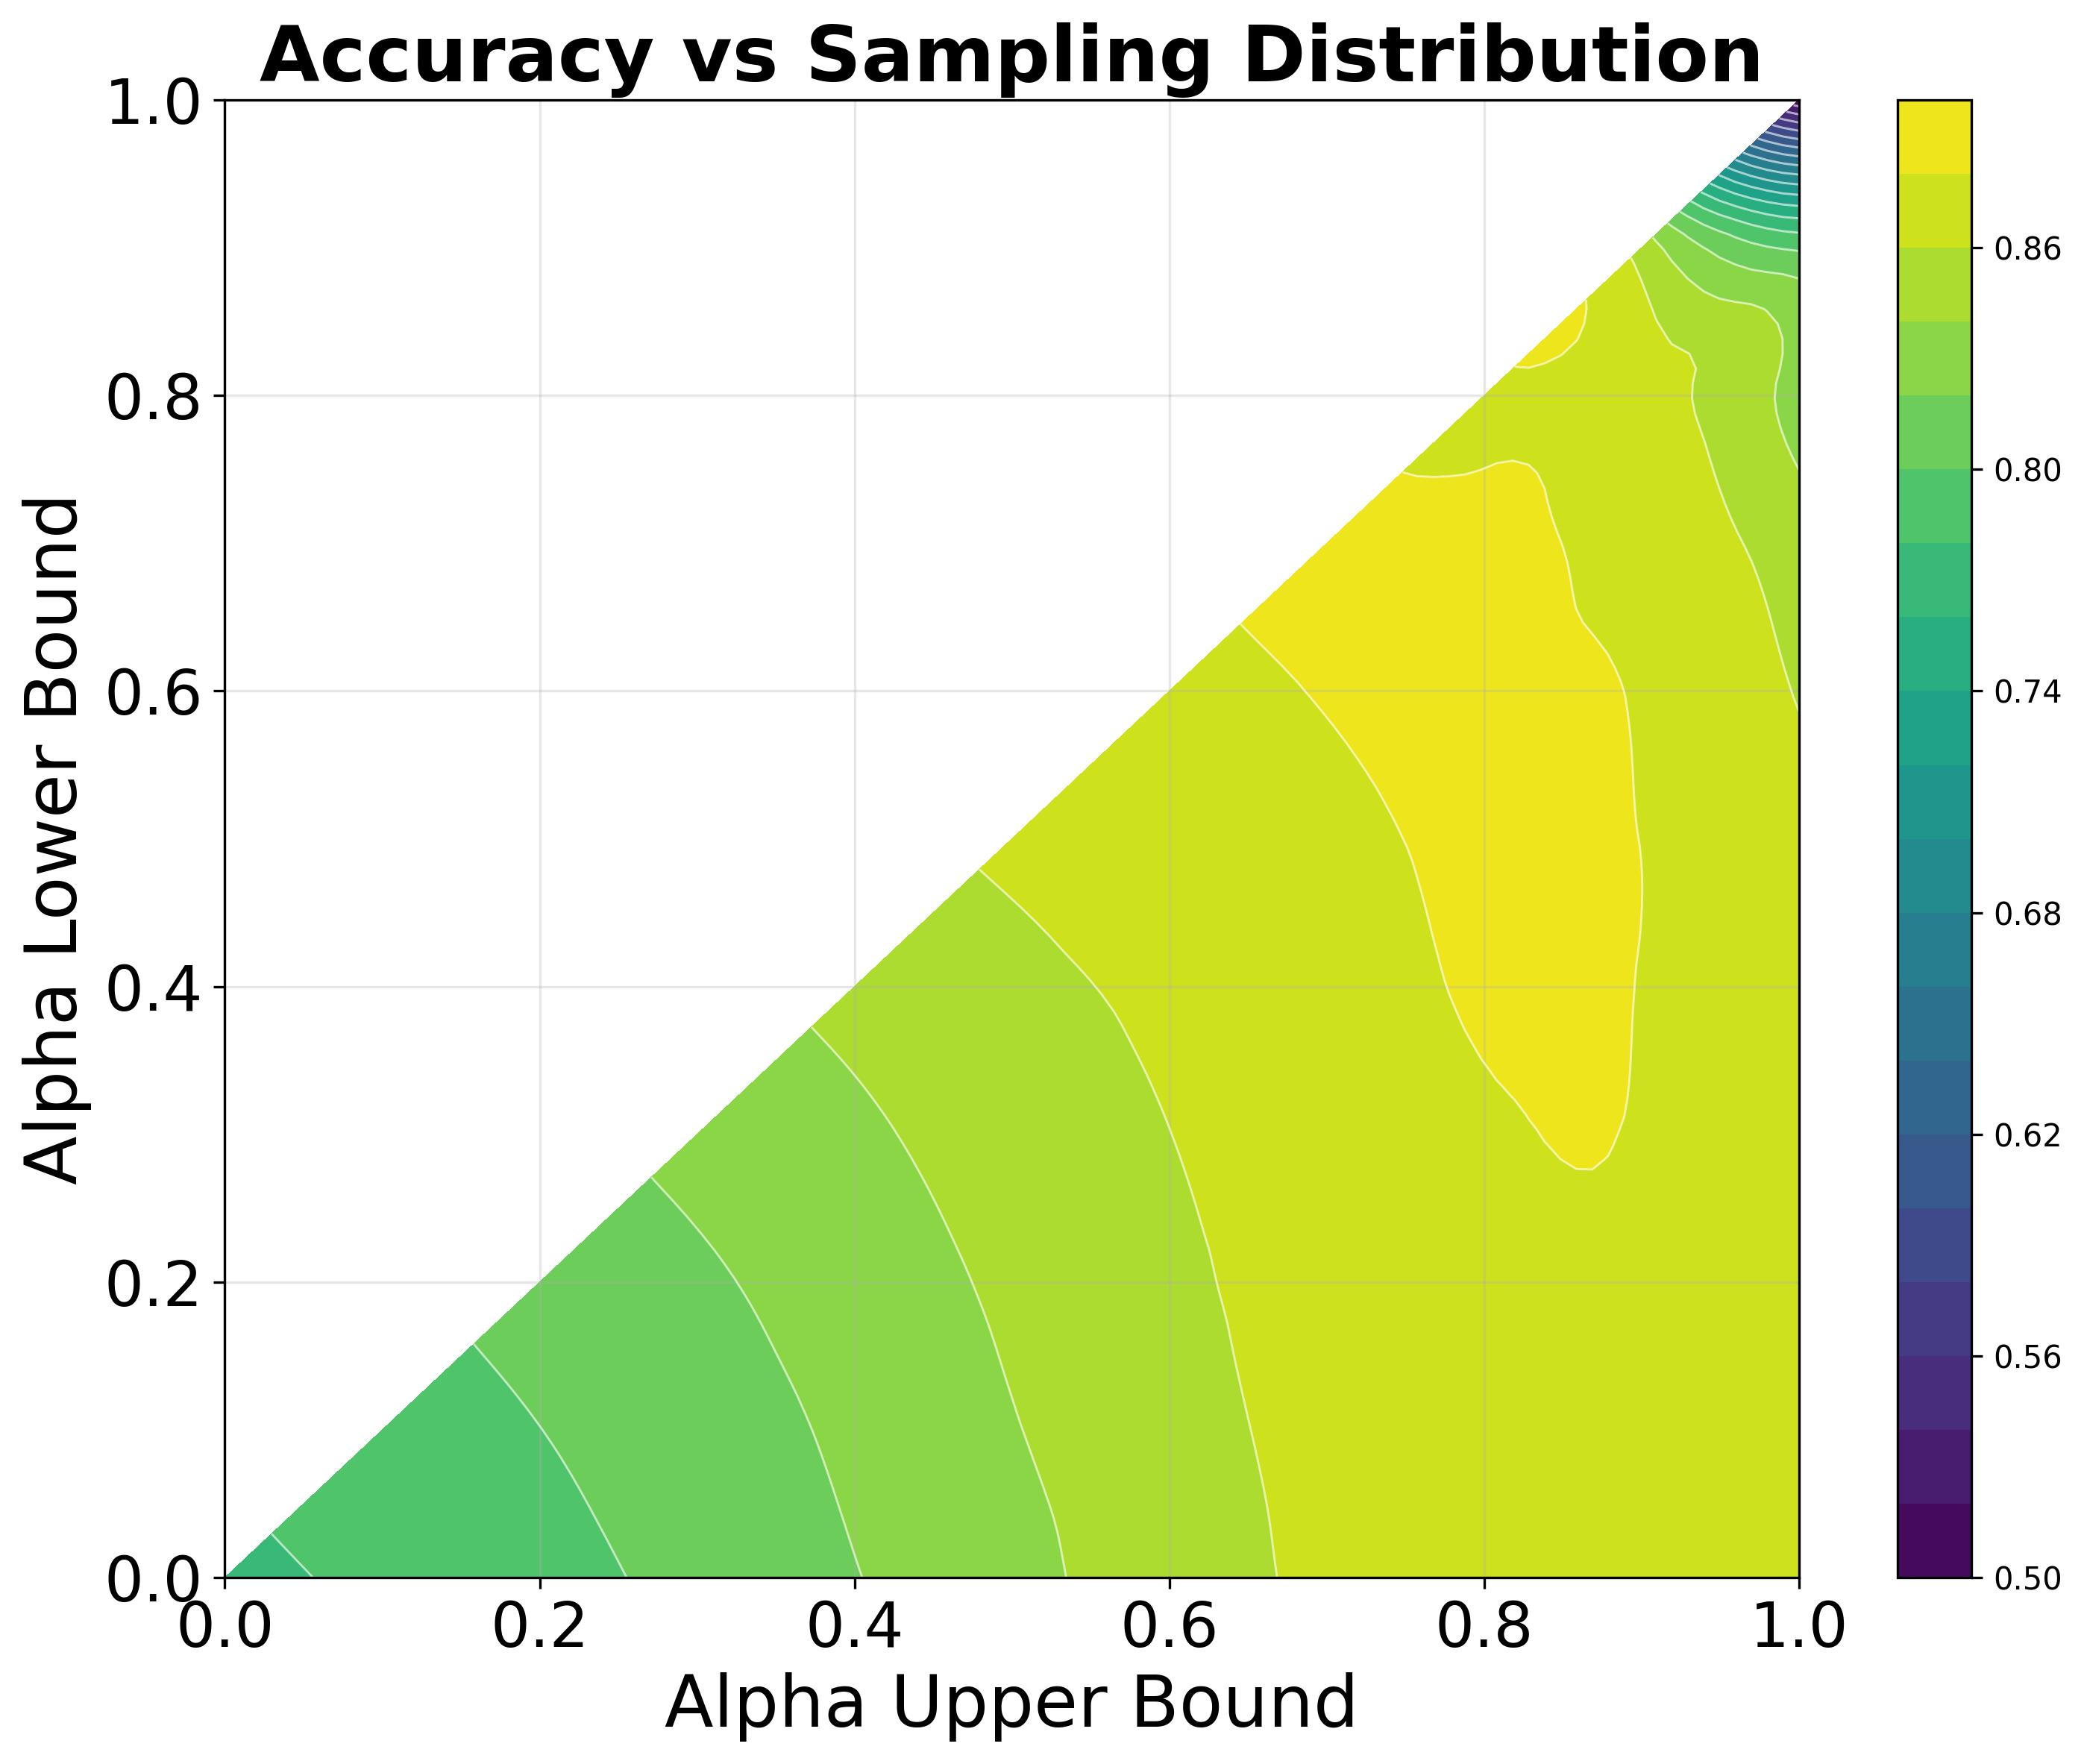
\includegraphics[width=\linewidth]{proposal/images/simlbr/alpha_ablation.jpeg}\\
  {\small (a)}
\end{minipage}\hfill
\begin{minipage}[t]{0.48\linewidth}
  \centering
  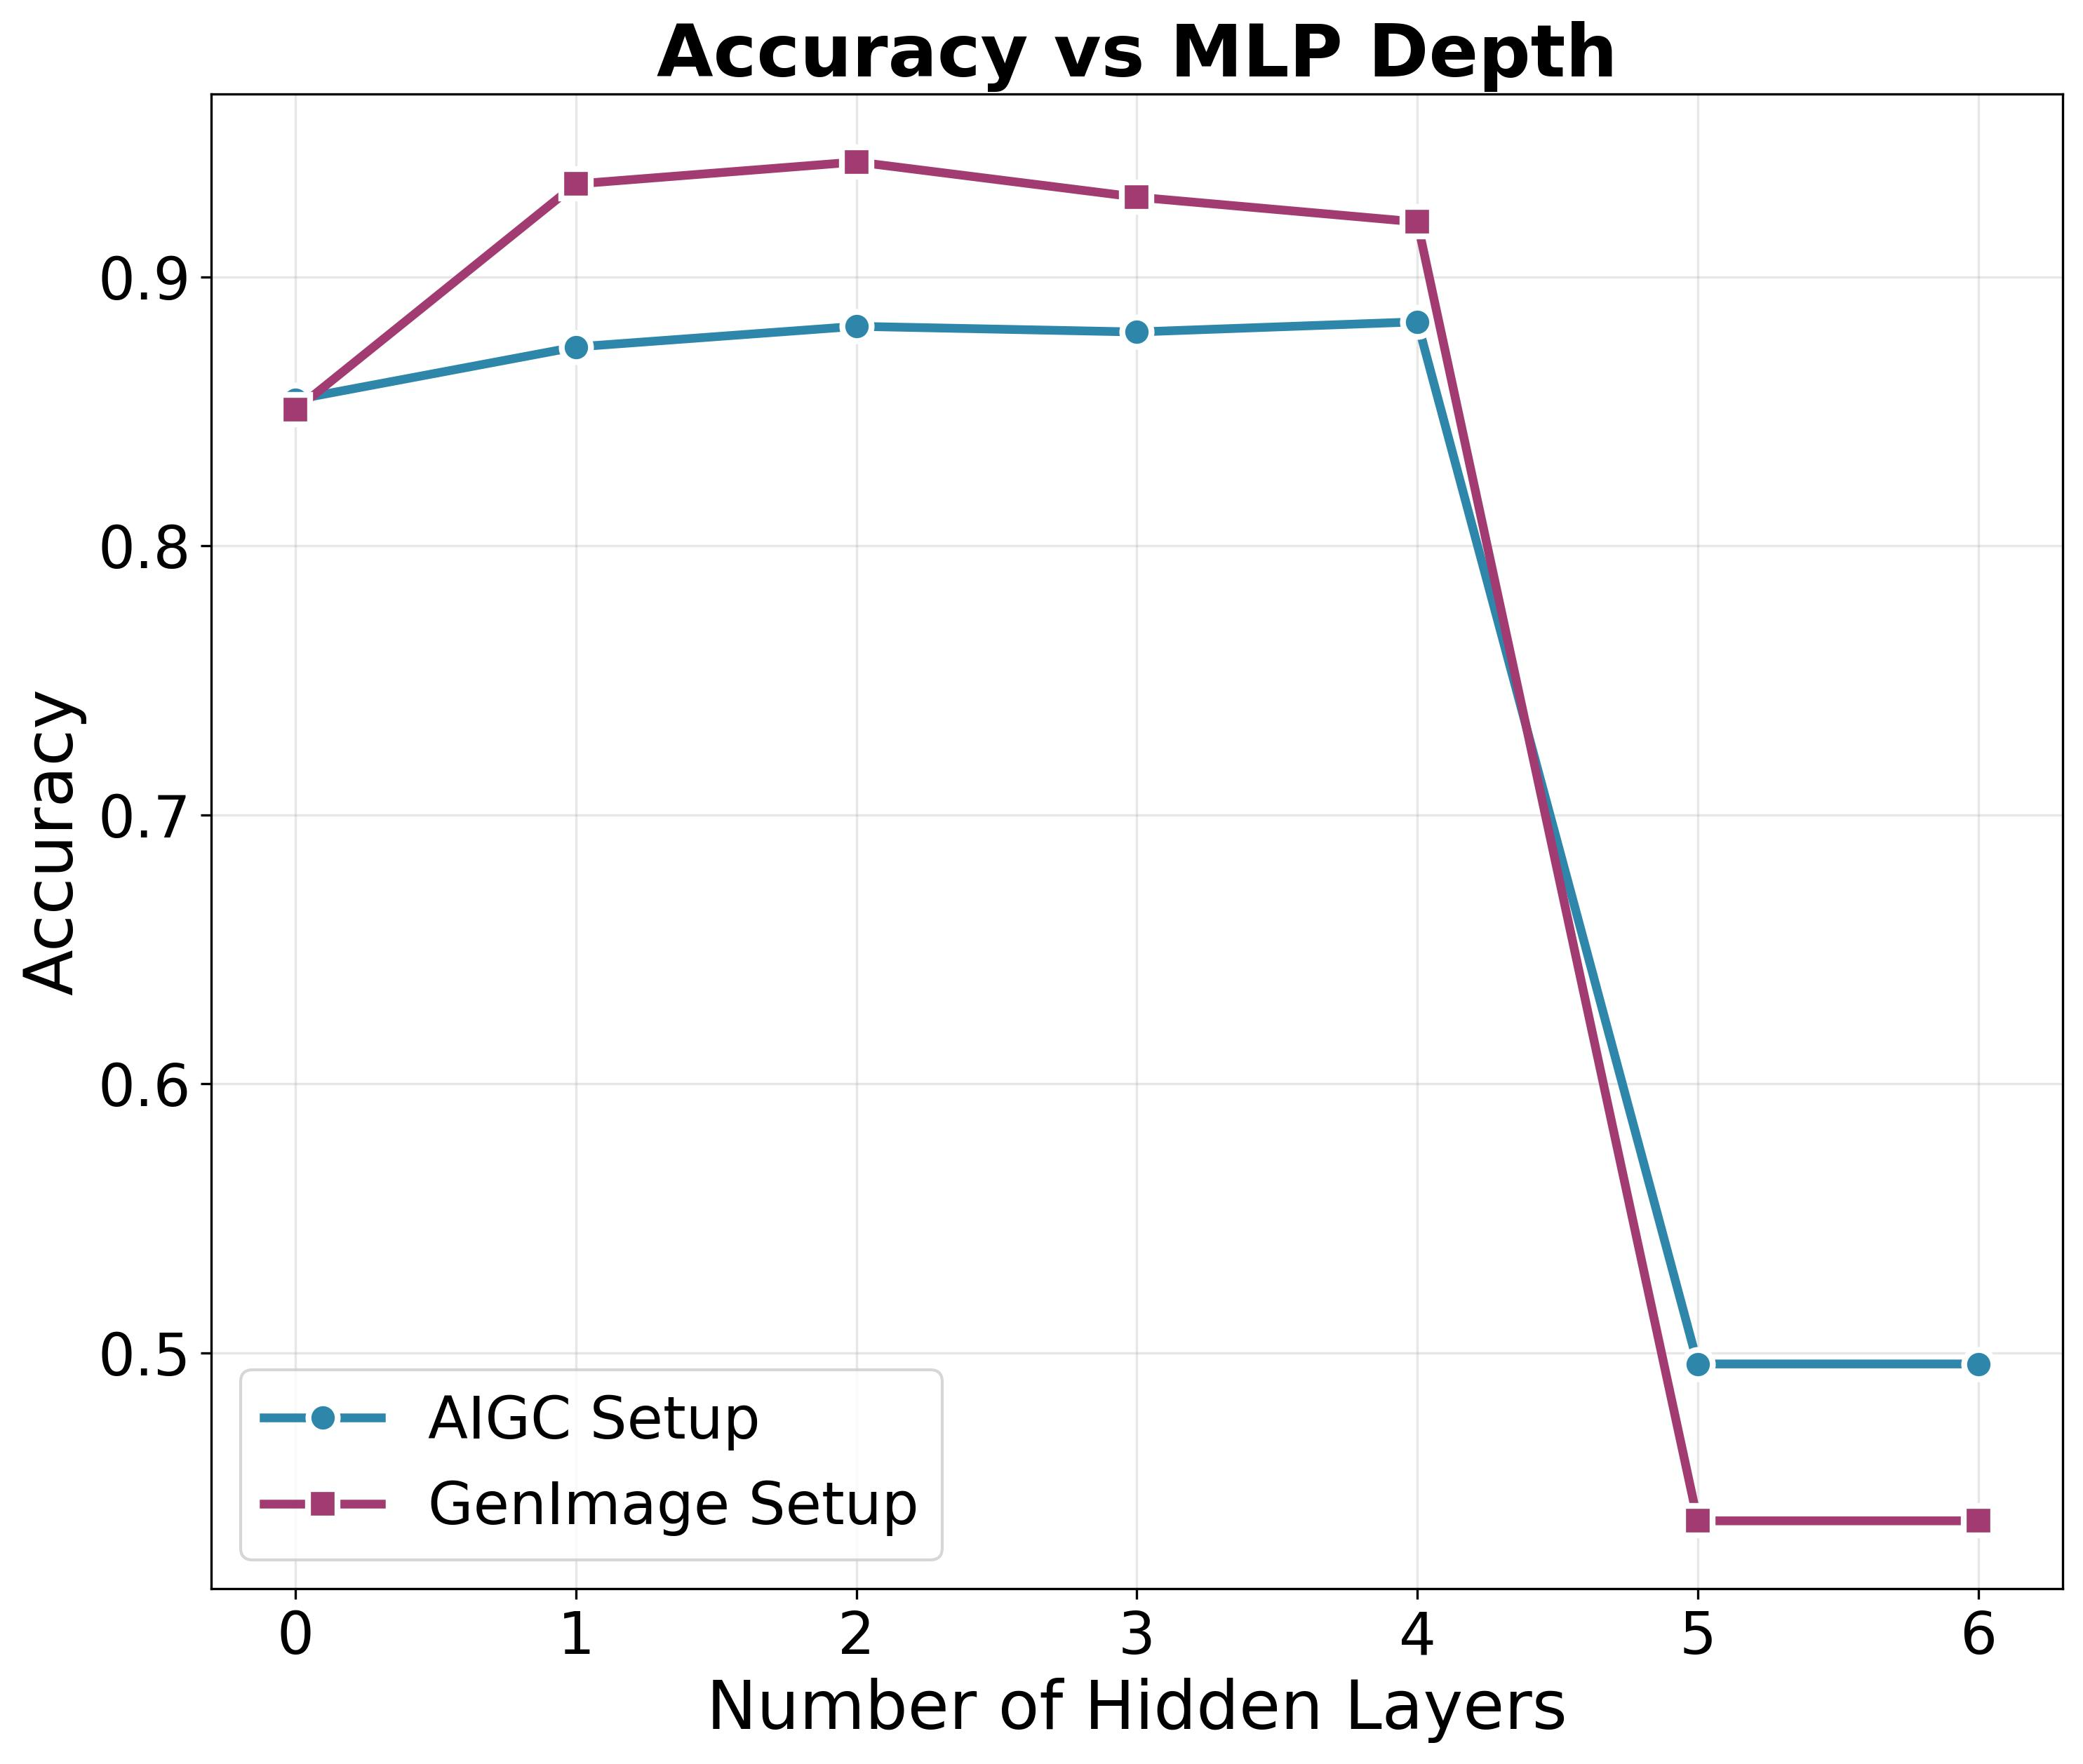
\includegraphics[width=\linewidth]{proposal/images/simlbr/depth_ablation.jpeg}\\
  {\small (b)}
\end{minipage}
\caption{\textbf{(a) Ablation of the sampling distribution for $\alpha$:} SimLBR is trained on ProGAN with different sampling distributions for $\alpha$. Always retaining at least half of the information from the real image is an optimal and robust choice. \textbf{(b) Ablation of MLP depth:} SimLBR performs better with smaller MLPs and overfits when the MLP has many hidden layers.}
\label{fig:simlbr_alpha_depth}
\end{figure}

\subsubsection{Ablation Studies}
\label{sec:simlbr_ablation}
\noindent\textbf{Impact of LBR and the latent space:} To isolate the contribution of latent blending regularization, we train a baseline MLP under an identical setup without LBR. To understand the role of the latent space, we also train models on features from the older DINOv2~\cite{oquab2024dinov2}. In addition to Chameleon, AIGC, and GenImage, this ablation includes RSFake-1M, which lets us evaluate the effect of LBR under a large shift in the image distribution. Since a satellite-specific DINOv2 is not available, RSFake-1M is evaluated only with the DINOv3 backbone. Table~\ref{table:simlbr_ablate} summarizes the results. Adding LBR in the DINOv3 latent space yields an average accuracy gain of $10.21\%$. The effect is even more pronounced for fake image accuracy, which improves from $7.24\%$ to $75.80\%$ on Chameleon (ProGAN), $54.07\%$ to $82.07\%$ on AIGC, $89.03\%$ to $92.96\%$ on Chameleon (SD v1.4), $85.80\%$ to $93.89\%$ on GenImage, and $48.28\%$ to $78.87\%$ on RSFake-1M, an average increase of over 25 percentage points. On RSFake-1M, the overall accuracy improves from $73.90\%$ to $88.88\%$, showing that LBR is equally effective for generated satellite imagery. LBR also substantially reduces the standard deviation across settings and improves the reliability and worst-case estimates.

Interestingly, LBR does not yield the same improvements in the DINOv2 latent space. LBR operates entirely in the latent space by injecting small amounts of fake information into real image latents. This assumes a geometrically smooth manifold, on which such interpolation yields a smooth change that stays on the valid embedding manifold. We hypothesize that the lack of improvement with DINOv2 is related to limitations in the manifold structure of weaker embedding models~\cite{kang2025clip,li2025lost,liu2024assessing}.

\noindent\textbf{In-distribution vs.\ out-of-distribution generators:} Detectors generally perform better on generators that share architectural similarities with the training generator, because these generators produce similar artifacts~\cite{zhu2023genimage,yansanity}. To further isolate the contribution of LBR, we partition the test generators into in-distribution (ID) and out-of-distribution (OD) groups. For AIGC, which is trained on ProGAN, GAN-based generators are ID and diffusion-based generators are OD; for GenImage, which is trained on Stable Diffusion, the assignment is reversed. Table~\ref{table:simlbr_idod} shows that LBR yields modest gains on ID generators, where the baseline already performs well, but large gains on OD generators ($10.30\%$ on GenImage and $12.72\%$ on AIGC). This shows that LBR helps the detector generalize beyond artifact-level correlations to previously unseen generative architectures.

\noindent\textbf{Sampling distribution for $\alpha$:} Figure~\ref{fig:simlbr_alpha_depth}(a) shows how different sampling strategies for $\alpha$ affect performance. Consistent with our hypothesis, sampling only low values of $\alpha$ leads to poor performance, since injecting excessive fake information makes the task trivial. Sampling only high values of $\alpha$ also degrades performance sharply, because the perturbed samples become nearly identical to unperturbed real images, which makes the regularization too strong. Sampling from $\text{Uniform}(0.5, B)$ balances these extremes, and the method is robust to the choice of $B$, with values in the range $0.7 < B < 0.9$ consistently yielding the best performance.

\noindent\textbf{MLP depth:} Figure~\ref{fig:simlbr_alpha_depth}(b) shows that SimLBR performs well with 0 to 4 hidden layers, but deteriorates rapidly beyond 4 layers, as larger MLPs overfit to the training data.

\noindent\textbf{Comparison to anomaly detection:} We train a One-Class SVM with an RBF kernel on DINOv3 features of the real training images, sweeping $\nu$ to find the best value. The OC-SVM performs substantially worse than SimLBR on both AIGC and GenImage. Modern generators produce photorealistic images whose latent representations lie close to those of real images, so learning the support of the real distribution alone is insufficient. SimLBR instead uses controlled amounts of fake information to shape a meaningful boundary around the real-image manifold. \todo{Decide whether to include the OC-SVM figures (proposal/images/simlbr/ocsvm\_aigc.png and ocsvm\_genimage.png) and report their numbers here.}

\noindent\textbf{Visualizing the learned embeddings:} Figure~\ref{fig:simlbr_tsne} shows t-SNE visualizations of the penultimate-layer embeddings of detectors trained on ProGAN with and without LBR. Without LBR, the detector overfits to the training fakes and does not preserve a meaningful separation between real and fake distributions; there is even a clear separation between the train and test real images. With LBR, the real images form a compact cluster, and fake images from the unseen generator fall outside it.

\subsection{Structured Latent Blending Regularization}
\label{sec:structured_lbr}
SimLBR constructs each pseudo-fake by moving a real embedding along a single direction, the line from $L^R$ to $L^F$, by a single scalar amount $\alpha$. As a result, the set of pseudo-fakes that can be created from a given real-fake pair is a line segment. In this section, we describe extensions of SimLBR that we developed after its publication. Each extension creates harder and more diverse pseudo-fakes by perturbing the real embedding along a richer set of directions. \todo{Add context: where and when this work was done (internship), collaborators, and its publication status.}

\noindent\textbf{Motivation:} LBR aims to create pseudo-fakes that lie just outside the real distribution. However, it does so by moving the global summary vector of the entire real image toward a fake. Any perturbation of the summary vector could move the latent significantly away from the real image distribution, making the pseudo-fake too easy to detect. One natural alternative, which we call Localized Latent Blending Regularization (LLBR), is to perturb only the local (patch-level) feature vectors rather than the summary vector, producing harder pseudo-fakes. \todo{State whether LLBR experiments were run and what they showed.} The geometric intuition behind LLBR is that the pseudo-fakes are created by moving along more diverse directions. This raises the question of whether the same intuition can be applied directly in the space of the global (CLS) representation, by perturbing only a subset of its dimensions.

\begin{figure}[!t]
\centering
\begin{minipage}[t]{0.52\linewidth}
  \centering
  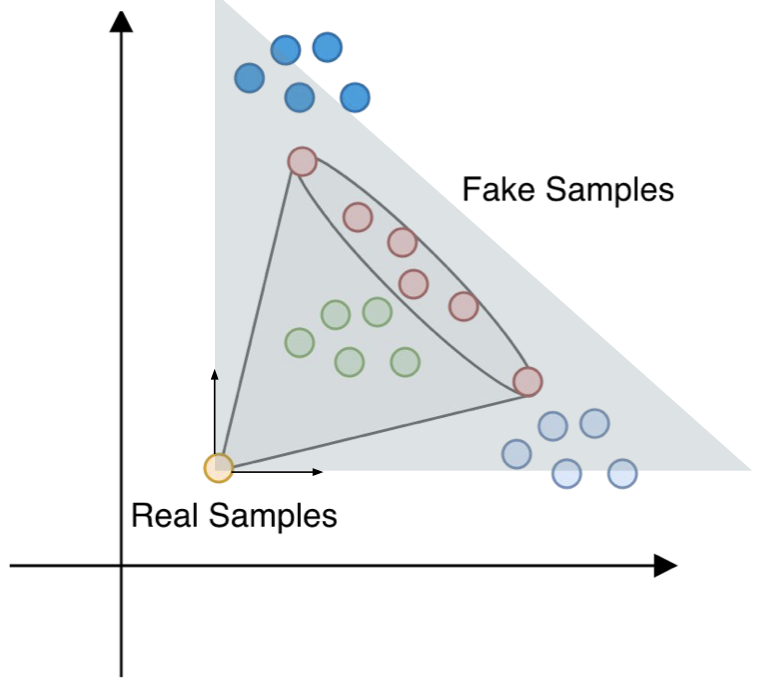
\includegraphics[width=\linewidth]{proposal/images/simlbr/plbr_geometry.png}\\
  {\small (a)}
\end{minipage}\hfill
\begin{minipage}[t]{0.42\linewidth}
  \centering
  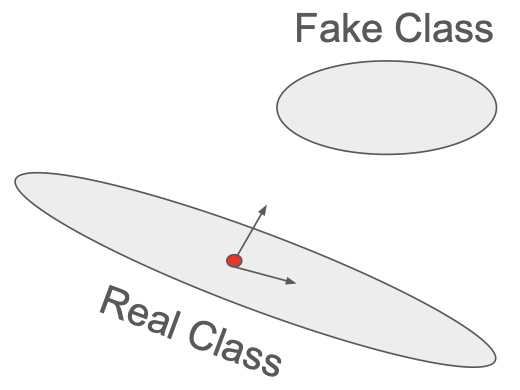
\includegraphics[width=\linewidth]{proposal/images/simlbr/pca_lbr_schematic.png}\\
  {\small (b)}
\end{minipage}
\caption{\textbf{Geometric intuition for structured LBR:} (a) SimLBR creates pseudo-fakes along the line segment between a real sample (yellow) and a fake sample (red). Perturbing different subsets of dimensions with different amounts expands the set of reachable pseudo-fakes (green) from a line segment to a larger region, covering more of the space in which unseen fakes (blue) may lie. (b) In a PCA basis of the real class, we know which directions have high and low variance, and can choose which directions to perturb. \todo{Redraw both panels for the dissertation; these are taken from presentation slides.}}
\label{fig:structured_lbr}
\end{figure}

\subsubsection{Partial Latent Blending Regularization (P-LBR)}
In Partial LBR, we blend only a subset of the dimensions of the latent representation. Let $d$ be the dimension of the representation, and let $\mathcal{S} \subset \{1, \ldots, d\}$ be a randomly sampled subset of $k$ dimensions. We define a per-dimension blending vector $\boldsymbol{\alpha} \in \mathbb{R}^d$ as:
\begin{equation}
\alpha_j =
\begin{cases}
\alpha, & j \in \mathcal{S}\\
1, & j \notin \mathcal{S}
\end{cases}
\qquad \alpha \sim \text{Uniform}(a, B)
\label{eq:plbr_alpha}
\end{equation}
The pseudo-fake representation is then computed as:
\begin{equation}
L_i = \boldsymbol{\alpha} \odot L_i^{R} + (\mathbf{1}-\boldsymbol{\alpha}) \odot L_i^{F}
\label{eq:plbr}
\end{equation}
where $\odot$ is the element-wise product. Dimensions outside $\mathcal{S}$ are copied unchanged from the real representation. SimLBR is the special case $k=d$. As illustrated in Figure~\ref{fig:structured_lbr}(a), because a different subset of dimensions is perturbed for each sample, the pseudo-fakes are no longer restricted to the line between $L^R$ and $L^F$. \todo{Confirm: the embedding dimension $d$, whether $\mathcal{S}$ is resampled for every training sample, and the final values of $k$, $a$, and $B$ (the best run used $k=712$, $\alpha \sim \text{Uniform}(0.6, 0.8)$, and weight decay \texttt{5e-3}).}

\subsubsection{Independent Latent Blending Regularization (I-LBR)}
P-LBR allows movement along only a subset of dimensions. In Independent LBR, we allow movement along all dimensions, but each dimension is blended by an independently sampled amount:
\begin{equation}
\alpha_j \sim \text{Uniform}(a, B) \quad \text{independently for } j = 1, \ldots, d
\label{eq:ilbr_alpha}
\end{equation}
with the pseudo-fake computed using Equation~\ref{eq:plbr}. This expands the feasible set of pseudo-fakes for a given real-fake pair from a line segment (SimLBR) to an axis-aligned hyperrectangle. The feasible set of pseudo-fakes from P-LBR is a subset of the feasible set of I-LBR when the same range of $\alpha$ is used. \todo{Confirm the final I-LBR configuration (the best run used $\alpha_j \sim \text{Uniform}(0.75, 0.8)$, weight decay \texttt{5e-3}, and a plateau learning-rate schedule).}

\subsubsection{PCA Latent Blending Regularization (PCA-LBR)}
Both P-LBR and I-LBR show that there is value in perturbing different dimensions by different amounts (Section~\ref{sec:structured_lbr_results}). However, they still rely on randomness to choose which dimensions to perturb. In PCA-LBR, we instead choose the perturbation directions using the structure of the data. We transform the representations to a new basis using PCA. In this basis, we know the directions of most and least variance of the data, and we use this information to decide which directions should be perturbed (Figure~\ref{fig:structured_lbr}(b)). Specifically:
\begin{enumerate}
    \item We compute supervised PCA between the real and fake classes and obtain the most discriminative direction $v_0$.
    \item We project the real data onto the orthogonal complement of $v_0$, i.e., we remove the $v_0$ component.
    \item We perform PCA on the projection of the real class onto $\text{span}\{v_0\}^\perp$, completing a basis $\mathcal{B} = \{v_0, v_1, \ldots, v_{d-1}\}$ with change-of-basis matrix $B$, where $v_1, \ldots, v_{d-1}$ are ordered by decreasing variance.
    \item We apply $B$ to all representations.
    \item For each real-fake pair $(r, f)$ in the new basis, we blend the coordinates for $v_0$ and for the $m$ lowest-variance directions $v_{d-m}, \ldots, v_{d-1}$. Let $\alpha_j^{\text{PCA}} = \alpha$ if $v_j$ is a direction to perturb and $\alpha_j^{\text{PCA}} = 1$ otherwise. The pseudo-fake is:
    \begin{equation}
    \boldsymbol{\alpha}^{\text{PCA}} \odot r + (\mathbf{1} - \boldsymbol{\alpha}^{\text{PCA}}) \odot f
    \label{eq:pcalbr}
    \end{equation}
    and it is labeled as fake. The classifier is trained in the space with basis $\mathcal{B}$.
\end{enumerate}
Perturbing the low-variance directions of the real class creates pseudo-fakes that leave the real distribution along directions in which real images rarely vary, which should make them both close to the real distribution and clearly distinct from it. \todo{Confirm: what ``supervised PCA'' refers to exactly, and the final number of perturbed directions $m$ for the PCA-PLBR results (runs are labeled ``partial712d-randomordered'').}

\begin{table}[!t]
\centering
\small
\begin{tabular}{l|ccc}
\hline
Generator & SimLBR & P-LBR & PCA-PLBR \\
\hline
ProGAN (Training) & 99.24 & \textbf{99.29} & 99.24 \\
\hline
StyleGAN   & 88.66 & 88.92 & \textbf{89.54} \\
BigGAN     & 95.75 & 95.30 & \textbf{95.80} \\
CycleGAN   & 89.36 & 88.19 & \textbf{90.84} \\
StarGAN    & 89.27 & \textbf{89.69} & 87.47 \\
GauGAN     & 96.98 & 97.06 & \textbf{97.52} \\
StyleGAN2  & 85.67 & 87.01 & \textbf{87.29} \\
WFIR       & 89.25 & \textbf{90.70} & 90.35 \\
ADM        & 85.81 & 86.08 & \textbf{86.85} \\
Glide      & 90.53 & 91.38 & \textbf{91.72} \\
Midjourney & 74.55 & \textbf{76.56} & 74.30 \\
SD v1.4    & 84.95 & \textbf{86.34} & 85.09 \\
SD v1.5    & 84.16 & \textbf{85.25} & 84.08 \\
VQDM       & 93.25 & 92.71 & \textbf{93.59} \\
Wukong     & 90.23 & \textbf{90.70} & 90.12 \\
DALLE2     & 79.80 & \textbf{82.65} & 81.20 \\
\hline
\textit{Mean}$\uparrow$        & 88.59 & \textbf{89.24} & 89.06 \\
\textit{Std}$\downarrow$         & 6.26 & \textbf{5.57} & 6.25 \\
\textit{Reliability}$\uparrow$ & 6.16 & \textbf{7.05} & 6.25 \\
\textit{WCE}$\uparrow$         & 74.55 & \textbf{76.56} & 74.30 \\
\hline
\end{tabular}
\caption{\textbf{Structured LBR on AIGC:} Accuracy of detectors trained on ProGAN. The SimLBR column is our re-run of SimLBR under the same setup as the structured variants. P-LBR improves mean accuracy, reliability, and the worst-case estimate over SimLBR. \todo{Explain why the re-run SimLBR mean (88.59) differs slightly from the published value (88.40).}}
\label{table:structured_aigc}
\end{table}

\begin{table}[!t]
\centering
\small
\begin{tabular}{l|cc}
\hline
Generator & SimLBR & PCA-PLBR \\
\hline
SD v1.4 (Training) & \textbf{97.54} & 97.23 \\
\hline
Midjourney & 92.46 & \textbf{92.52} \\
SD v1.5    & \textbf{97.66} & 97.26 \\
ADM        & \textbf{96.15} & 95.43 \\
GLIDE      & 92.95 & \textbf{93.48} \\
Wukong     & \textbf{97.24} & 96.88 \\
VQDM       & 93.74 & \textbf{94.14} \\
BigGAN     & 88.94 & \textbf{90.65} \\
\hline
\textit{Mean}$\uparrow$        & 94.59 & \textbf{94.70} \\
\textit{Std}$\downarrow$         & 3.10 & \textbf{2.43} \\
\textit{Reliability}$\uparrow$ & 14.36 & \textbf{18.41} \\
\textit{WCE}$\uparrow$         & 88.94 & \textbf{90.65} \\
\hline
\end{tabular}
\caption{\textbf{Structured LBR on GenImage:} Accuracy of detectors trained on Stable Diffusion v1.4. PCA-PLBR improves the accuracy on the most out-of-distribution generator, BigGAN, which reduces the variance across generators and improves the reliability and worst-case estimate.}
\label{table:structured_genimage}
\end{table}

\begin{table}[!t]
\centering
\begin{tabular}{l|ccc}
\hline
Method & Accuracy & Real Acc. & Fake Acc. \\
\hline
SimLBR       & 84.33 & 90.74 & 75.80 \\
P-LBR        & 83.84 & 89.30 & \textbf{76.58} \\
PCA-PLBR     & \textbf{84.92} & \textbf{92.98} & 74.19 \\
\hline
\end{tabular}
\caption{\textbf{Structured LBR on Chameleon:} Detectors are trained on ProGAN.}
\label{table:structured_chameleon}
\end{table}

\subsubsection{Experiments and Results}
\label{sec:structured_lbr_results}
We follow the experimental setup of SimLBR and train all variants on DINOv3 features. During development, we compared variants by their validation accuracy when trained on AIGC (ProGAN). \todo{Specify which validation split was used for model selection.}

\noindent\textbf{Development experiments:} Perturbing a random subset of $512$ dimensions with P-LBR did not improve over SimLBR (peak validation accuracy of approximately $88.0\%$ for both). Increasing the subset to $704$ or $712$ dimensions improved the peak validation accuracy to approximately $88.4\%$. Narrowing the sampling range of $\alpha$ to $\text{Uniform}(0.6, 0.8)$ and reducing the weight decay to \texttt{5e-3} further improved it to approximately $88.7\%$, our best P-LBR configuration. I-LBR reached a similar peak validation accuracy of approximately $88.7\%$, without a clear advantage over P-LBR. \todo{Replace the approximate values read from the training curves with the exact logged numbers.}

\noindent\textbf{Low-variance vs.\ high-variance directions:} To test the intuition behind PCA-LBR, we reversed the selection and perturbed the \textit{highest}-variance directions instead of the lowest. Perturbing low-variance directions was consistently better: with 256 perturbed directions, the peak validation accuracy was approximately $87.4\%$ for low-variance directions vs.\ $86.9\%$ for high-variance directions; with 512 directions, approximately $87.5\%$ vs.\ $87.2\%$; and with 712 directions, approximately $88.4\%$ vs.\ $88.3\%$. This supports the hypothesis that pseudo-fakes are more useful when they leave the real distribution along directions in which real images rarely vary.

\noindent\textbf{AIGC:} Table~\ref{table:structured_aigc} reports the full evaluation on AIGC. P-LBR improves the mean accuracy from $88.59\%$ to $89.24\%$ and gives the largest improvements on generators where SimLBR is weakest, such as DALLE2 ($+2.85\%$), Midjourney ($+2.01\%$), and Stable Diffusion v1.4 ($+1.39\%$). As a result, P-LBR reduces the standard deviation from $6.26$ to $5.57$, improves the reliability from $6.16$ to $7.05$, and raises the worst-case estimate from $74.55\%$ to $76.56\%$. PCA-PLBR improves the mean accuracy to $89.06\%$, with gains on most GAN-based generators, but does not improve the worst-case estimate.

\noindent\textbf{GenImage:} Table~\ref{table:structured_genimage} compares SimLBR and PCA-PLBR on GenImage. The mean accuracy is nearly unchanged ($94.59\%$ vs.\ $94.70\%$), but PCA-PLBR improves the accuracy on BigGAN, the generator most different from the training generator, from $88.94\%$ to $90.65\%$. This reduces the standard deviation from $3.10$ to $2.43$ and improves the reliability from $14.36$ to $18.41$.

\noindent\textbf{Chameleon:} Table~\ref{table:structured_chameleon} shows the results on Chameleon. PCA-PLBR achieves the highest overall accuracy ($84.92\%$), driven by better real-image accuracy ($92.98\%$), while P-LBR achieves the highest fake-image accuracy ($76.58\%$).

\noindent\textbf{Discussion:} The structured variants of LBR give consistent but modest improvements over SimLBR. The improvements in mean accuracy are under one percentage point, but they are concentrated on the hardest, most out-of-distribution generators, which translates into larger improvements in reliability and in the worst-case estimate. This supports the geometric intuition that moving real embeddings along more diverse, and more carefully chosen, directions produces pseudo-fakes that better define the boundary of the real distribution. A natural next step is to select the perturbed directions and their blending amounts using the eigenvalues of the real class, rather than a fixed number of lowest-variance directions.


\subsection{Proposed Direction}
In this section, we outline the next steps planned for this chapter. In Section~\ref{sec:few-shot}, we conducted few-shot learning experiments on geospatial deepfakes and proposed two hypotheses from the results. We plan to validate these hypotheses with experimental results. For H1, we will design visualization pipelines to inspect the artifacts in the deepfake qualitatively. For H2, we will utilize the representations extracted from deepfakes to train downstream models and investigate how this impacts performance when compared to using uncorrupted training data. 

In Section~\ref{sec:seperability}, we proposed a new metric, $Seperability@K$, to measure the presence of artifacts in deepfakes. We will compute this metric for the state-of-the-art geospatial generative models. We will rank the models based on our metric and analyze the correlation with other generative metrics such as LPIPS and FID scores. 

In Section~\ref{sec:simlbr}, we presented SimLBR, a simple and efficient framework for generalizable fake image detection that learns a tight decision boundary around the real image distribution using latent blending regularization, and in Section~\ref{sec:structured_lbr}, we extended it with structured perturbations that move real embeddings along more diverse and more carefully chosen directions. A remaining direction is to use SimLBR as a feedback mechanism for generative models to improve the $Separability$ score of these models. A better generative model can feed into pretraining pipelines to scale and learn richer and more generalizable representations. \todo{Update this section once the status of the few-shot hypotheses, the Separability metric, soft-label learning, and the generative-model feedback work is decided.}

\subsection{Chapter Conclusion}
In summary, these are the major tasks required to complete this chapter:
\begin{itemize}
    \item Design a framework to validate the hypotheses offered in Section~\ref{sec:few-shot}.
    \item Run experiments to compute $ Separability$ scores for state-of-the-art models. Validate the utility of our proposed metrics.
    \item Develop SimLBR, a generalizable fake image detector based on latent blending regularization, and extend it with structured latent blending (Sections~\ref{sec:simlbr} and~\ref{sec:structured_lbr}). \textit{(Completed.)}
    \item Work towards using the results from this chapter to improve geospatial generative models and feed good quality data to improve representation learning pipelines.
\end{itemize}
\newpage
\section{Timeline}
\begin{table}[!h]
\resizebox{\linewidth}{!}{
\begin{tabular}{llllllllllllllll}
\hline
 \multicolumn{1}{|l|}{} & \multicolumn{8}{c|}{2025}                                                                                                                                                                                                                   & \multicolumn{7}{c|}{2026}                                                           \\
\hline
\multicolumn{1}{|l|}{}                                                                                    & \multicolumn{1}{l|}{May} & \multicolumn{1}{l|}{Jun} & \multicolumn{1}{l|}{Jul} & \multicolumn{1}{l|}{Aug} & \multicolumn{1}{l|}{Sep} & \multicolumn{1}{l|}{Oct} & \multicolumn{1}{l|}{Nov}                      & \multicolumn{1}{l|}{Dec} & \multicolumn{1}{l|}{Jan} & \multicolumn{1}{l|}{Feb} & \multicolumn{1}{l|}{Mar} & \multicolumn{1}{l|}{Apr} & \multicolumn{1}{l|}{May} & \multicolumn{1}{l|}{Jun} & \multicolumn{1}{l|}{Jul} \\ \hline
\multicolumn{1}{|l|}{Internship}                                                                          & \multicolumn{4}{l|}{\cellcolor[HTML]{FFCE93}}                                                             & \multicolumn{1}{l|}{}    & \multicolumn{1}{l|}{}    & \multicolumn{1}{l|}{}                         & \multicolumn{1}{l|}{}    & \multicolumn{1}{l|}{}    & \multicolumn{1}{l|}{}    & \multicolumn{1}{l|}{}    & \multicolumn{1}{l|}{}    & \multicolumn{1}{l|}{}    & \multicolumn{1}{l|}{}    & \multicolumn{1}{l|}{}    \\ \hline
\multicolumn{1}{|l|}{Few-shot experiments}                                                                & \multicolumn{1}{l|}{}    & \multicolumn{1}{l|}{}    & \multicolumn{3}{l|}{\cellcolor[HTML]{CBCEFB}}                                  & \multicolumn{1}{l|}{}    & \multicolumn{1}{l|}{}                         & \multicolumn{1}{l|}{}    & \multicolumn{1}{l|}{}    & \multicolumn{1}{l|}{}    & \multicolumn{1}{l|}{}    & \multicolumn{1}{l|}{}    & \multicolumn{1}{l|}{}    & \multicolumn{1}{l|}{}    & \multicolumn{1}{l|}{}    \\ \hline
\multicolumn{1}{|l|}{Initial SimDLR framework}                                                            & \multicolumn{1}{l|}{}    & \multicolumn{1}{l|}{}    & \multicolumn{1}{l|}{}    & \multicolumn{2}{l|}{\cellcolor[HTML]{CBCEFB}}       & \multicolumn{1}{l|}{}    & \multicolumn{1}{l|}{}                         & \multicolumn{1}{l|}{}    & \multicolumn{1}{l|}{}    & \multicolumn{1}{l|}{}    & \multicolumn{1}{l|}{}    & \multicolumn{1}{l|}{}    & \multicolumn{1}{l|}{}    & \multicolumn{1}{l|}{}    & \multicolumn{1}{l|}{}    \\ \hline
\multicolumn{1}{|l|}{Work on dissertation proposal}                                                       & \multicolumn{1}{l|}{}    & \multicolumn{1}{l|}{}    & \multicolumn{1}{l|}{}    & \multicolumn{3}{l|}{\cellcolor[HTML]{FFFFC7}}                                  & \multicolumn{1}{l|}{}                         & \multicolumn{1}{l|}{}    & \multicolumn{1}{l|}{}    & \multicolumn{1}{l|}{}    & \multicolumn{1}{l|}{}    & \multicolumn{1}{l|}{}    & \multicolumn{1}{l|}{}    & \multicolumn{1}{l|}{}    & \multicolumn{1}{l|}{}    \\ \hline
\multicolumn{1}{|l|}{Seperability metric}                                                                 & \multicolumn{1}{l|}{}    & \multicolumn{1}{l|}{}    & \multicolumn{1}{l|}{}    & \multicolumn{1}{l|}{}    & \multicolumn{3}{l|}{\cellcolor[HTML]{CBCEFB}}                                                       & \multicolumn{1}{l|}{}    & \multicolumn{1}{l|}{}    & \multicolumn{1}{l|}{}    & \multicolumn{1}{l|}{}    & \multicolumn{1}{l|}{}    & \multicolumn{1}{l|}{}    & \multicolumn{1}{l|}{}    & \multicolumn{1}{l|}{}    \\ \hline
\multicolumn{1}{|l|}{\begin{tabular}[c]{@{}l@{}}Experimental validation of\\ hypotheses\end{tabular}}     & \multicolumn{1}{l|}{}    & \multicolumn{1}{l|}{}    & \multicolumn{1}{l|}{}    & \multicolumn{1}{l|}{}    & \multicolumn{1}{l|}{}    & \multicolumn{2}{l|}{\cellcolor[HTML]{CBCEFB}}                            & \multicolumn{1}{l|}{}    & \multicolumn{1}{l|}{}    & \multicolumn{1}{l|}{}    & \multicolumn{1}{l|}{}    & \multicolumn{1}{l|}{}    & \multicolumn{1}{l|}{}    & \multicolumn{1}{l|}{}    & \multicolumn{1}{l|}{}    \\ \hline
\multicolumn{1}{|l|}{New adjustments to SimDLR}                                                           & \multicolumn{1}{l|}{}    & \multicolumn{1}{l|}{}    & \multicolumn{1}{l|}{}    & \multicolumn{1}{l|}{}    & \multicolumn{1}{l|}{}    & \multicolumn{4}{l|}{\cellcolor[HTML]{CBCEFB}}                                                                                  & \multicolumn{1}{l|}{}    & \multicolumn{1}{l|}{}    & \multicolumn{1}{l|}{}    & \multicolumn{1}{l|}{}    & \multicolumn{1}{l|}{}    & \multicolumn{1}{l|}{}    \\ \hline
\multicolumn{1}{|l|}{\begin{tabular}[c]{@{}l@{}}Submit SimDLR and Sat360 \\ to CVPR 2026\end{tabular}}                                                           & \multicolumn{1}{l|}{}    & \multicolumn{1}{l|}{}    & \multicolumn{1}{l|}{}    & \multicolumn{1}{l|}{}    & \multicolumn{1}{l|}{}    & \multicolumn{1}{l|}{}    & \multicolumn{1}{l|}{\cellcolor[HTML]{34ff34}} & \multicolumn{1}{l|}{}    & \multicolumn{1}{l|}{}    & \multicolumn{1}{l|}{}    & \multicolumn{1}{l|}{}    & \multicolumn{1}{l|}{}    & \multicolumn{1}{l|}{}    & \multicolumn{1}{l|}{}    & \multicolumn{1}{l|}{}    \\ \hline

\multicolumn{1}{|l|}{\begin{tabular}[c]{@{}l@{}}Using SimDLR to improve \\ generative models\end{tabular}} & \multicolumn{1}{l|}{}    & \multicolumn{1}{l|}{}    & \multicolumn{1}{l|}{}    & \multicolumn{1}{l|}{}    & \multicolumn{1}{l|}{}    & \multicolumn{1}{l|}{}    & \multicolumn{1}{l|}{}                         & \multicolumn{1}{l|}{}    & \multicolumn{4}{l|}{\cellcolor[HTML]{CBCEFB}}                                     & \multicolumn{1}{l|}{}    & \multicolumn{1}{l|}{}    & \multicolumn{1}{l|}{}    \\ \hline
\multicolumn{1}{|l|}{Deadline for ECCV 2026}                                                           & \multicolumn{1}{l|}{}    & \multicolumn{1}{l|}{}    & \multicolumn{1}{l|}{}    & \multicolumn{1}{l|}{}    & \multicolumn{1}{l|}{}    & \multicolumn{1}{l|}{}    & \multicolumn{1}{l|}{} & \multicolumn{1}{l|}{}    & \multicolumn{1}{l|}{}    & \multicolumn{1}{l|}{}    & \multicolumn{1}{l|}{\cellcolor[HTML]{34ff34}}    & \multicolumn{1}{l|}{}    & \multicolumn{1}{l|}{}    & \multicolumn{1}{l|}{}    & \multicolumn{1}{l|}{}    \\ \hline
\multicolumn{1}{|l|}{Write and defend dissertation}                                                       & \multicolumn{1}{l|}{}    & \multicolumn{1}{l|}{}    & \multicolumn{1}{l|}{}    & \multicolumn{1}{l|}{}    & \multicolumn{1}{l|}{}    & \multicolumn{1}{l|}{}    & \multicolumn{1}{l|}{}                         & \multicolumn{1}{l|}{}    & \multicolumn{1}{l|}{}    & \multicolumn{1}{l|}{}       & \multicolumn{5}{l|}{\cellcolor[HTML]{FFFFC7}}                                                             \\ \hline
\end{tabular}
}
\caption{Proposed timeline to complete dissertation.}
\end{table}
    
    



